\documentclass[
uplatex,
b5paper,
10pt,
%english,
dvipdfmx
]{jsbook}

\usepackage{type1cm} % 任意サイズの拡大縮小を可能にする
\usepackage{nruby}
\usepackage[dvipdfmx]{hyperref}
\usepackage{pxjahyper}
\hypersetup{% hyperrefオプションリスト
 setpagesize=false,
 bookmarksnumbered=true,%
 bookmarksopen=true,%
 colorlinks=true,%
 linkcolor=black,
 urlcolor=black,
 citecolor=red,
}

\usepackage{framed}
\usepackage{wrapfig}
\usepackage{scalefnt}
\usepackage{version,url,here}	% required for `\comment' (yatex added)
\usepackage[dvipdfmx]{graphicx}	% required for `\includegraphics' (yatex added)
\usepackage{natbib,url}
\usepackage{pdfpages}
%\usepackage[varg]{txfonts}
\usepackage{makeidx}
%\usepackage{listings,jlisting}
\usepackage{listings,plistings}
\usepackage{color}
%\usepackage{xcolor}
\lstloadlanguages{[LaTeX]TeX, sh}
\colorlet{lstcolTeX}{green!50!black}
\colorlet{lstcoltext}{black}
\colorlet{lstcolshell}{blue!50!black}

\newcounter{marginparcntbw}[chapter]
\newcommand{\theMarginparcntbw}{$\dagger$\arabic{marginparcntbw}}
\newcommand{\Marginparbw}[2][−10pt]{%
  \stepcounter{marginparcntbw}%
  \textsuperscript{\theMarginparcntbw}%
  \protect\marginpar{\vskip#1\footnotesize%
    \textsuperscript{\theMarginparcntbw}
    {#2}\par}}


\setlength{\fboxsep}{.5zw}
\setlength{\fboxrule}{.6pt}

\begin{comment}
\lstset{basicstyle=\small\ttfamily, keywordstyle={}, commentstyle={},
  columns=flexible, showspaces=false, showstringspaces=false,
  aboveskip=12pt, belowskip=12pt, frame=tb,
  framesep=8pt, framerule=2pt, xleftmargin=10pt,
  xrightmargin=10pt, framexleftmargin=10pt, framexrightmargin=10pt
}
\end{comment}

\lstdefinestyle{shell}{language=sh, rulecolor=\color{lstcolshell!25}}
\lstdefinestyle{TeX}{language=TeX, rulecolor=\color{lstcolTeX!25}}
\lstdefinestyle{text}{language=TeX, rulecolor=\color{lstcoltext!25}}
\begin{comment}
\lstnewenvironment{listing}[1][]
{\lstset{#1}}
{}
\end{comment}


\lstset{% 
language={C++}, 
% backgroundcolor={\color[gray]{.85}},% 
basicstyle={\small},% 
identifierstyle={\small},% 
%commentstyle={\small\ttfamily \color[rgb]{0,0.5,0}},% 
%keywordstyle={\small\bfseries \color[rgb]{0,0,1}},% 
ndkeywordstyle={\small},% 
stringstyle={\small\ttfamily}, 
frame={tb}, 
breaklines=true, 
columns=[l]{fullflexible},% 
numbers=left,% 
xrightmargin=0zw,% 
xleftmargin=3zw,% 
numberstyle={\scriptsize},% 
stepnumber=1, 
numbersep=1zw,% 
morecomment=[l]{//}% 
} 

\begin{comment}
\lstset{
    basicstyle={\ttfamily\footnotesize}, %書体の指定
    keywordstyle={\footnotesize\ttfamily},%
%    frame=tRBl, %フレームの指定
    frame={t}, %フレームの指定
    framerule=1.2pt, %フレームの指定     
%    frame=leftbar, %フレームの指定
    framesep=0pt, %フレームと中身(コード)の間隔
    breaklines=true, %行が長くなった場合の改行
    linewidth=1\textwidth, %フレームの横幅
    xrightmargin=3zw,%
    xleftmargin=3zw,%
    numbers=left,%
    numberstyle={\ttfamily\scriptsize},%
    lineskip=0\baselineskip, %行間の調整
    tabsize=2 %Tabを何文字幅にするかの指定
}
\end{comment}

%\usepackage[format=hang,labelsep=colon,margin=10pt,sc,small]{caption}
\bibpunct[:\,]{(}{)}{,}{a}{}{,}
\definecolor{royalblue}{rgb}{0.0, 0.14, 0.4}
\newcommand{\colorrule}[1]{%
\begingroup\color{#1}\hrule\endgroup%
}%
\newcommand{\Colorrule}[1]{%
\begingroup\color{#1}\rule{1\textwidth}{2.4pt}\endgroup%
}%
\newcommand{\TColorrule}[1]{%
\begingroup\color{#1}\rule[2pt]{1\textwidth}{.6pt}\endgroup%
}%

\usepackage{framed}
\usepackage{color}
\usepackage{dcolumn}
\newcolumntype{d}[1]{D{.}{.}{#1}}
\usepackage{multicol}

\definecolor{lightgray}{rgb}{0.75,0.75,0.75}

\newtheorem{theo}{定理}[section]
\newtheorem{defi}{定義}[section]
\newtheorem{lemm}{補題}[section]

\makeatletter
\renewenvironment{leftbar}{%
%  \def\FrameCommand{\vrule width 3pt \hspace{10pt}}%  デフォルトの線の太さは3pt
  \def\FrameCommand{\vrule width 1pt \hspace{10pt}}% 
  \MakeFramed {\advance\hsize-\width \FrameRestore}}%
 {\endMakeFramed}
\makeatother

\newenvironment{redleftbar}{%
  \def\FrameCommand{\textcolor{red}{\vrule width 1pt} \hspace{10pt}}% 
  \MakeFramed {\advance\hsize-\width \FrameRestore}}%
 {\endMakeFramed}

\newenvironment{lightgrayleftbar}{%
  \def\FrameCommand{\textcolor{lightgray}{\vrule width .5zw} \hspace{10pt}}% 
  \MakeFramed {\advance\hsize-\width \FrameRestore}}%
{\endMakeFramed}


\AtBeginDvi{\special{papersize=\the\paperwidth,\the\paperheight}}

\newcommand{\mini}[2]{%
\setbox0=\hbox{\tt#1}\dp0=4pt%
\setbox1=\hbox{\tiny#2}\ht1=4pt\dp1=7pt%
\leavevmode\vtop{\offinterlineskip\box0\box1}}


\newif\ifVOLONE
\newif\ifVOLTWO
\newif\ifVOLTHREE

\VOLONEtrue
\VOLTWOfalse
\VOLTHREEfalse

% Japanese用の条件マクロ
\newif\ifJapanese
\newif\ifEnglish
%\Japanesefalse
\Japanesetrue   

% English用の条件マクロ
\ifJapanese
\renewcommand{\lstlistlistingname}{プログラム一覧}
\Englishfalse
\else
\Englishtrue
\fi

\newif\ifBLANK
%\BLANKtrue
\BLANKfalse

\newif\ifBIB
%\BIBtrue
\BIBfalse

\newif\ifINDEX
\INDEXtrue
%\INDEXfalse

\newif\ifOUT
%\OUTtrue
\OUTfalse

\newif\ifSHADOW
%\SHADOWtrue
\SHADOWfalse

\newif\ifSchedule
%\Scheduletrue
\Schedulefalse

\newif\ifBook
%\Booktrue
\Bookfalse

\newif\ifPreface
\Prefacetrue
%\Prefacefalse


\newif\ifCHSummary
%\CHSummarytrue
\CHSummaryfalse

\newif\ifPOSTSCRIPT
%\POSTSCRIPTtrue
\POSTSCRIPTfalse

\newif\ifWORKBOOK
\WORKBOOKtrue
%\WORKBOOKfalse


\newif\ifPLAYGAME
%\PLAYGAMEtrue
\PLAYGAMEfalse

\newif\ifVOCAB
%\VOCABtrue
\VOCABfalse

\newif\ifDEVELOPPER
%\DEVELOPPERtrue
\DEVELOPPERfalse

\ifWORKBOOK
\DEVELOPPERfalse
\Prefacetrue
\Booktrue
\CHSummaryfalse
\fi



\newcounter{excount}
\setcounter{excount}{0}
\newcounter{kdcount}
\setcounter{kdcount}{0}
\newcounter{ancount}
\setcounter{ancount}{0}
\newcounter{columncnt}
\setcounter{columncnt}{0}


\ifBook
\newenvironment{toiquestion}{%
\vspace{-1\baselineskip}
\noindent
\refstepcounter{excount}
\begin{quote}%
 \bfseries 
 \hspace{-2zw}問\theexcount\hspace{.7zw}%
}{%
\end{quote}
%\vspace{1.5\baselineskip}
%\vspace{-.5\baselineskip}
}
\else
\newenvironment{toiquestion}{%
\vspace{-1\baselineskip}
\noindent
\refstepcounter{excount}
\begin{quote}%
 \hspace{-2zw}問\theexcount\hspace{.7zw}%
}{%
\end{quote}
%\vspace{1\baselineskip}
%\vspace{-.5\baselineskip}
}
\fi

\newenvironment{toianswer}{%
%\vspace{-2\baselineskip}%
 \begin{quote}
  \parindent=1zw
  \hspace{.6zw}%
}{%
 \end{quote}
}

\setlength\unitlength{1pt}


\ifEnglish
\title{{\LARGE Linguistics}\\\protect\Colorrule{red}\\{\normalsize In very common daily life}}
\author{Hilofumi Yamamoto\\{\small\sc Ph.\,D. in Linguistics}}
\date{Tokyo Institute of Technology}
\else
\title{言語学\\
\vspace{-.5\baselineskip}
\Colorrule{red}\\\normalsize ことば研究史}
\author{山 元 啓 史\\{\small Ph.\,D.\,in Linguistics}}
\date{東京工業大学}
\fi

\makeindex
\begin{document}
\frontmatter
%\maketitle
\thispagestyle{empty}
\setlength\unitlength{1pt}
\begin{picture}(150,70)(70,565)  
% \put(162,182){\fbox{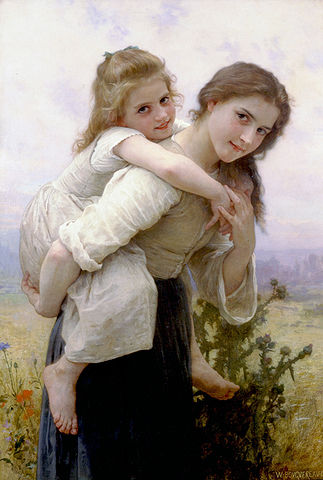
\includegraphics[trim=0 0 0 0,clip,width=0.52\hsize]{William-Bouguereau.jpg}}}
 \put( 0,475){\linethickness{0.4mm}\line(1,0){600}}
 \put( 0,173){\linethickness{0.4mm}\line(1,0){600}}
\ifEnglish
 \put(170,578){\scalefont{2.0}\bfseries Idiomatic Japanese}
 \put(145,555){\scalefont{1.5}\bfseries The Secret of Advanced Japanese}
 \put(230,530){\scalefont{1.8}\bfseries Volume 1}
% \put(210,500){\includegraphics[trim=10 45 10 45, clip, width=12mm]{./edx-logo.eps}}
 \put(245,502){\scalefont{1.5}\itshape\bfseries Tokyo\,Tech\,X}
 \put(100,484){\scalefont{1.5}\bfseries Let's learn Idiomatic Expressions of Japanese}
% \put(210,450){\scalefont{3.0} Workbook}
 \put(160,145){\scalefont{2.0}\bfseries Hilofumi Yamamoto}
 \put(215,130){\itshape\bfseries Ph.\,D.\,in Linguistics}
 \else
 \put(170,578){\scalefont{2.0}\bfseries Idiomatic Japanese}
 \put(145,555){\scalefont{1.5}\bfseries The Secret of Advanced Japanese}
 \put(230,530){\scalefont{1.8}\bfseries Volume 1}
 \put(100,484){\scalefont{1.5}\bfseries Let's learn Idiomatic Expressions of Japanese}

 \put(160,145){\scalefont{2.0}\bfseries Hilofumi Yamamoto}
 \put(215,130){\itshape\bfseries Ph.\,D.\,in Linguistics}

% \put(202,162){\scalefont{0.8}\bfseries やま}
% \put(239,162){\scalefont{0.8}\bfseries もと}
% \put(275,162){\scalefont{0.8}\bfseries ひろ}
% \put(312,162){\scalefont{0.8}\bfseries ふみ}
% \put(200,145){\scalefont{2.0}\bfseries 山 元 啓 史}
% \put(215,130){\itshape\bfseries Ph.\,D.\,in Linguistics}
\fi
\end{picture}
\newpage

\ifEnglish
Idiomatic Japanese, Volume 1
\else
日本語らしい日本語: 上級への道 Volume 1
\fi

\setlength\unitlength{1pt}
 \begin{picture}(0,130)(60,100)
  
%  \put(63,40){\fbox{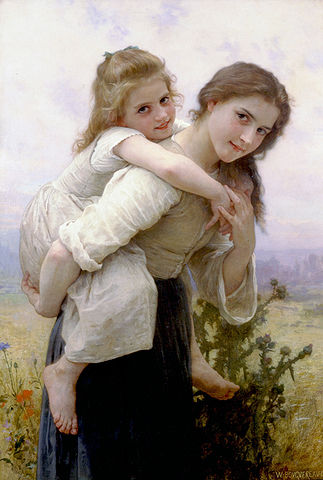
\includegraphics[trim=0 0 0 0,clip,width=0.3\hsize]{William-Bouguereau.jpg}}}  
%  \put(190,37){
\includegraphics[width=5mm]{./Cc-public_domain_mark_white.eps}}
  
% \ifEnglish
% \put(55,20){\scalefont{1.0} Fardeau agr\'eable (french for ``Pleasant Burden'')}
% \put(65,06){\scalefont{1.0} 1895 by William-Adolphe Bouguereau  (1825--1905)}
% \else
% \put(55,20){\scalefont{1.0} Fardeau agr\'eable (french for ``Pleasant Burden'')}
% \put(65,06){\scalefont{1.0} 1895 by William-Adolphe Bouguereau  (1825--1905)}
%\fi
 \end{picture}
% https://commons.wikimedia.org/wiki/File:Mary_Lemon_Waller_-_Spring_Voices_royalacademyillu1896roya_0070.jpg
\vfill

Hilofumi Yamamoto, Ph.\,D. in Linguistics, Tokyo Institute of Technology

\textcopyright\,Hilofumi Yamamoto, 2019


\ifPreface
\ifEnglish
\chapter*{Preface}
This book is one of the textbooks used in Institute of Science Tokyo’ ``Idiom Expressions in Japanese.''

There is a knack to learning languages.  
Do not get caught up in the details.  
Focus on expressions that are actually used in daily life.  
Not all conjugations of all verbs are used evenly.  
Even if a form is grammatically correct, some forms are never used in real communication because of their meaning.  
You do not need to study what is not used.

You can see which forms are used and which are not by observing real situations where the language is spoken.  
Rather than wondering *why* something is said in a particular way, try using it yourself.  
You will feel how naturally it fits.

No matter how much you study the structure of a bicycle, you will never learn to ride one.  
Many people can ride a bicycle without knowing anything about its structure.  
Just looking at a bicycle will not teach you to ride.  
The only way to learn is to actually ride it.  
So, let's try.
\else
\chapter*{はじめに}

本書は東京科学大学の教科書「日本語のイディオムと表現」である。
言語の勉強にはコツがあります。
詳細なところにこだわらないことである。
よく使われることだけ、勉強することである。
すべての動詞のすべての活用形が、均一に使われるわけではない。
文法的であったとしても、意味によって使われない形も存在する。
使われもしないものを勉強する必要はない。
どれが使われ、どれが使われないかは、その言語が話されている場面を見て確かめてみるとわかるだろう。
どうしてそう言うのだろうかと考えるよりも、その言い方を自分で使ってみると良いだろう。
その言い方がいかにフィットしているかがわかることだろう。

自転車の構造をいくら勉強しても、自転車には乗れない。
自転車の構造を知らないで自転車に乗っている人はたくさんいる。
自転車を見ているだけでは、自転車に乗れない。
とにかく自転車に乗らなければ、乗れるようにはなれない。
やってみよう。
\fi

\vspace*{1\baselineskip}
\begin{flushright}
 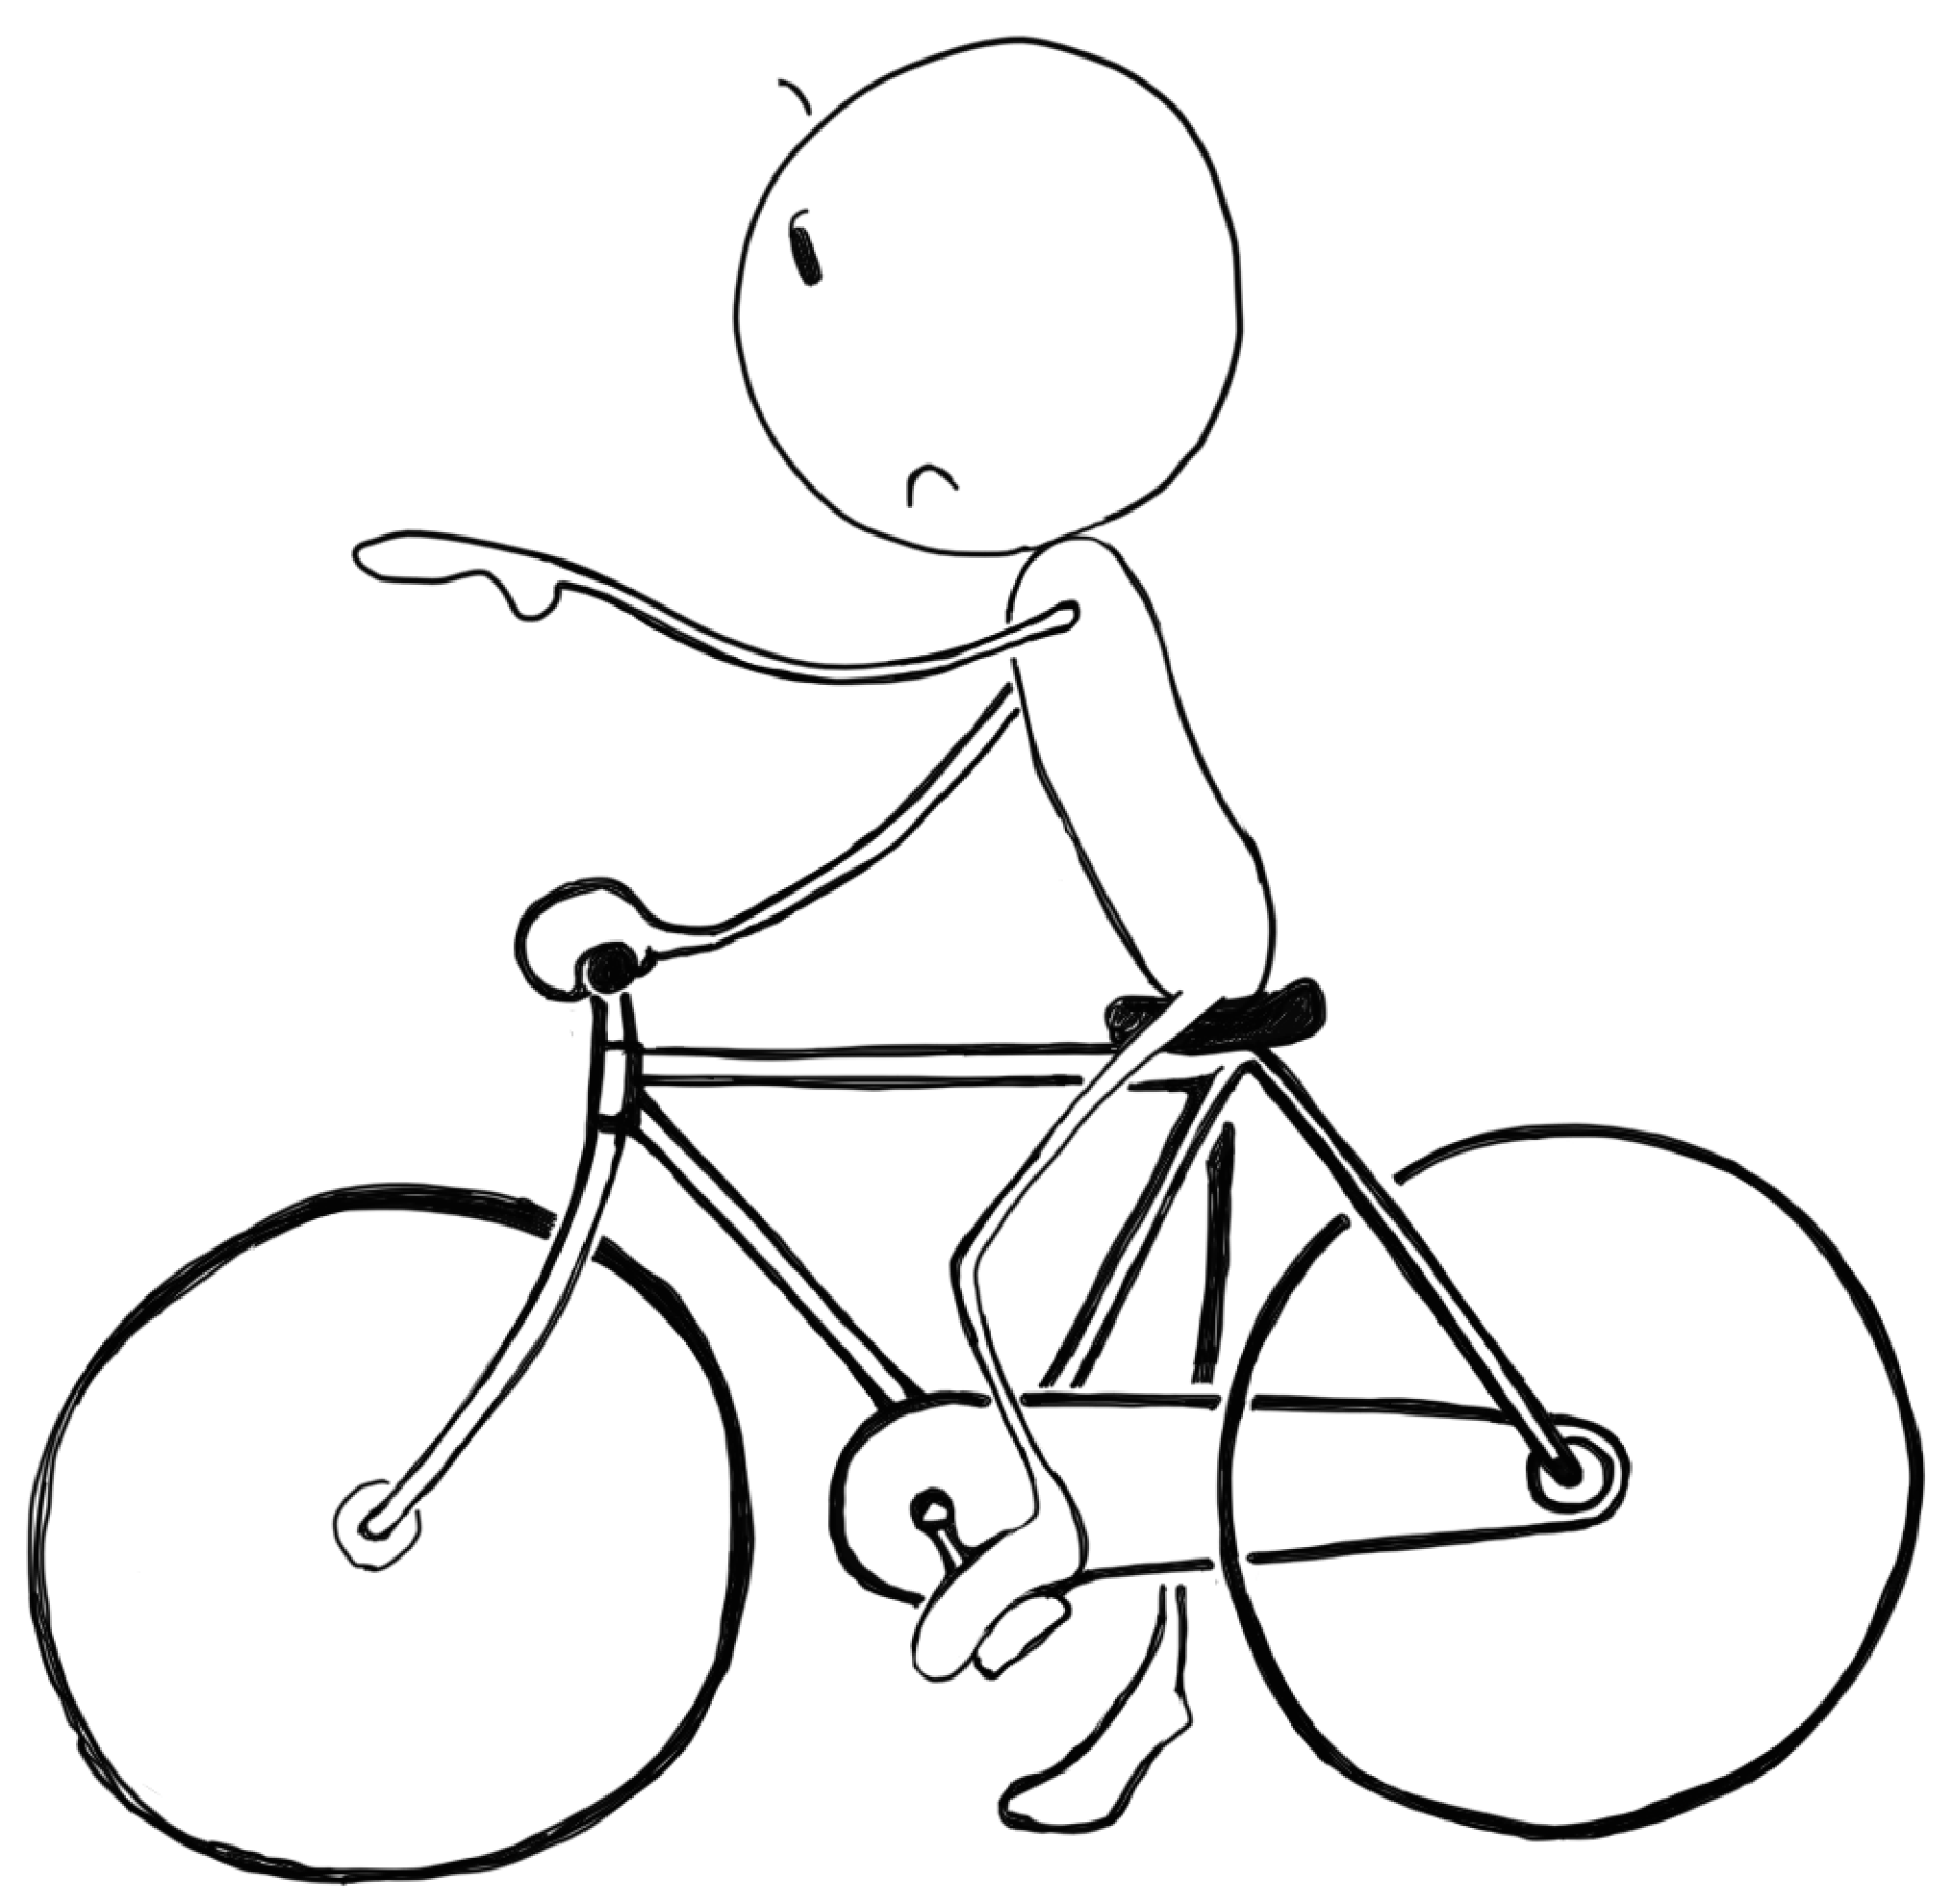
\includegraphics[width=.2\hsize]{bicycle201801.pdf}

 \ifEnglish
 Hilofumi Yamamoto, Ph.\,D.\\
 Professor of Linguistics\\
 Tokyo Institute of Technology\\
 \else
 {\large 山 元 啓 史}\hspace*{3zw}
 
 {\small 東京工業大学教授\hspace*{2zw}}
\fi
\end{flushright}

%\end{document} % for checking the first page.

\begin{comment}
\section*{Abbreviation}

\begin{multicols}{2}
\begin{description}
 \item[1G] 1st group verb
 \item[2G] 2nd group verb
 \item[3G] 3rd group verb
 \item[adj] adjective
 \item[adv] adverb
 \item[archaic] archaic word
 \item[casual] casual style
 \item[causa] causative
 \item[col] colloquial expression
 \item[v.comp] compound verb
 \item[n.comp] compound noun
 \item[cond] conditional form
 \item[formal] formal style
 \item[GN] grammar notes
 \item[honor] an honorific form of verb,
 \item[i-adj] i-adjective
 \item[n] noun
 \item[na-adj] na-adjective
 \item[non-past] non past tense
 \item[psiv] passive voice
 \item[past] past tense
 \item[pot] potential form
 \item[prefix] prefix
 \item[suffix] suffix
 \item[suru] suru verb
 \item[te-iru] te-iru
 \item[te-ita] te-iru
 \item[te-te] te-te
 \item[te-ta] te-ta
 \item[v.te] te-form of verb 
 \item[v] verb
 \item[vi] intransit verb 
 \item[voli] volitional form	    
 \item[vt] transit verb 
\end{description}
\end{multicols}
\end{comment}


\setcounter{tocdepth}{0}
\tableofcontents
%\listoffigures
%\listoftables
%\lstlistoflistings

\mainmatter

\ifEnglish
\chapter{Getting Started}
\else
\chapter{さあ、はじめよう}
\fi

\ifEnglish
\else
\fi


\includepdf[pages=12-21, scale=.84, trim=70 80 70 80, clip, offset=0mm -7mm, pagecommand={\thispagestyle{plain}}]{idiom_compact.pdf}
\label{113010_11Dec18} % U2S1


%%%%%%%%%%%%%%%%%%%%%%%%%%%%%%%%%%%%%%%%%%%%%%
%%   Presession  %%%%%%%%%%%%%%%%%%%%%%%%%%%%%
%%%%%%%%%%%%%%%%%%%%%%%%%%%%%%%%%%%%%%%%%%%%%%


%%%%%%%%%%%%%%%%%%%%%%%%%%%%%%%%%%%%%%%%%%%%%%
%%   Dictation   %%%%%%%%%%%%%%%%%%%%%%%%%%%%%
%%%%%%%%%%%%%%%%%%%%%%%%%%%%%%%%%%%%%%%%%%%%%%

\ifEnglish
\chapter{Commentary}

\else
\chapter{解説編}

\fi

例文、解説、小練習、関連事項を掲載した解説編である。
練習編と同様、10の表現が1回分として使えるようになっている。

%\section*{日本語のイディオムと文型: 1 -- 10}
\begin{enumerate}
\setcounter{enumi}{0}
%\setlength{\itemsep}{-4pt}

%1
\index{にかぎって@に限って}
\index{かぎる@限る}
\index{あてにならない@当てにならない}
\index{まるで@まるで}
 \item 傘を持って来ない日に\underline{ A }雨が降るから、天気予報はまる
       で\underline{ B }。

 \begin{itemize}
 % \itemsep=-4pt
  \item[□] A 限って; B 当てにならない
  \item[◆] 「〜に限って」〈その時はいつもちょうど悪く...  「限る」とは
	    一般的には「ある状況のときだけ」と条件を限定する。この場合、
	    実際は、「傘を持っていない時にだけ雨が降る」わけではないので
	    あるが、2〜3度でもそのようなことがあると、まるで傘を持って
	    いないときばかり雨が降るような悪いことがおこる気持ちがするも
	    ので、そのような気持ちを表す主観的な表現。
 \end{itemize}

 \begin{itemize}
% \itemsep=-4pt
  \item 予習していないときに限って、先生に当てられる。
  \item 忙しいときに限って、友達から電話がかかる。
  \item 勉強していないところに限って、試験にでる。
  \item 部屋が散らかっているときに限って、来客がある。
 \end{itemize}

「だけ」と比較
\index{だけ@だけ}
 \begin{itemize}
% \itemsep=-4pt
  \item 予習していないときだけ、先生に当てられる。(客観的事実)
  \item 忙しいときだけ、友達から電話がかかる。     (客観的事実)
 \end{itemize}

 \begin{itemize}
% \itemsep=-4pt
  \item[□] B 当てにならない 〈信用できない当たらない 〈的中しない
  \item[◆]「まるで」に二つの意味がある。この場合は「まったく〜ない」の意味。
 \end{itemize}

 \begin{itemize}
% \itemsep=-4pt
  \item まるで当てにならない(全然〜ない)
  \item まるで当たらない
  \item (よく似ている場合は) まるで人形のようにかわいい。
 \end{itemize}

▽他の答えの可能性チェック

 \begin{itemize}
% \itemsep=-4pt
  \item[○] よく:「しばしば」(運が悪いというくやしさはない。)
  \item[?] 必ず:100%の確率で (傘のない日はいつも)
  \item[?] いきなり:ある常識的な一連の経過をたどらないで、突然に行動をして相手を驚かせる様子
  \item いきなり結婚してほしいと言われてどうしていいかわからなかった。
  \item いい天気だったのに、いきなり降り出した。(曇ったりして降りそうな様子も見せずに)
  \item[?] 突然:急に。「いきなり」の方が、急に起こったことがらに不意打
	    ちを受けた気持ちが強い。「突然」は現象を客観的に表現。これに
	    対して「いきなり」は情意的。
  \item[?] もかかわらず:
  \item[○] デートの約束の日にもかかわらず、彼は残業した。 
  \item[×]        〃        彼はいつも残業する。
  \item デートの約束にかかわらず、彼はいつも残業する。
  \item 晴雨にかかわらず明日バザーをします。
  \item お酒を飲む飲まないにかかわらず、会費は500円です。
  \item この会は年齢にかかわらず、だれでも入会できます。
  \item[×] 雨にもかかわらず、あしたサッカーの試合をします。
  \item 〜にかかわらず(関係なく):規定でも未定でもいい
  \item 〜にもかかわらず:〈規定の事実〉にもかかわらず、〈規定〉
 \end{itemize}

       ※1の文が1回きりのある事実を述べる文なのか、一般的な事実として
       述べる文なのか考えて見よう。それによって、?のマークのついている
       ものの適、不適がわかるだろう。

%2
\index{ほど〜ない@ほど〜ない}
\index{ほど@ほど}
 \item 今日も寒いが、それでもきのうほど\underline{\hspace{3zw}}。

\begin{itemize}
% \itemsep=-4pt
\item[□] 寒くない
\item[◆] 文型「〜ほど...ない」。また、「が」の前が普通体であることか
	  ら考えて「寒くありませんでした」は誤りとなる。
\item[※] 「今日も」の「も」から「きのうも寒かった」を読み取ること、「き
	  のうほど」の「ほど」から比較した結果「...ではない」を予測でき
	  ることが必要。これが「きのうより」だったら、どうなるか。
\end{itemize}

\begin{itemize}
% \itemsep=-4pt
\index{より@より}
\item 今日も寒いが、それでもきのうより\underline{\hspace{3zw}}。
\item[→] 昨日と今日と単語を入れ換えたらどうなるか。
\item 昨日も寒かったが、それでも今日ほど\underline{\hspace{3zw}}。
\item[→] テンスに注意
\end{itemize}

%3
\index{からには@からには}
\index{から@から}
\item 私はやると言ったからには最後まで\underline{\hspace{3zw}}。

\begin{itemize}
% \itemsep=-4pt
\index{ぬく@ぬく}
\index{ふくごうどうし@複合動詞}
\item[□] やる/やりぬく/やらなければらならい/がんばる 等
\item[◆] 文型「〜からには...する」〈〜した以上は(そういう条件であるか
	  ら)、当然...する〉という意味。「〜から...する」〈〜ので(その
	  結果)、...する〉で「には」がはいると意味が異なってくる。
\item[▽] 他の答えの可能性チェック...やるべきだ/やるつもりだ/?やってみ
	  たい
\item[※] 「〜る(ます)」「〜ない(ません)」(意志動詞 非過去)の主語
	  が「私」の場合は強い意志表現となる。〜べきだ、〜つもりだの方が
	  より間接的な表現。
\end{itemize}

%4
\index{かかっている@かかっている}
\index{じどうしとたどうし@自動詞と他動詞}
\item 鍵が\underline{\hspace{3zw}}いるから、どこかへ出かけたのでしょう。

\begin{itemize}
% \itemsep=-4pt
\item[□] 掛かって
\item[◆] 自動詞と他動詞の使い方に注意
\end{itemize}

\begin{itemize}
% \itemsep=-4pt
\item 鍵がかかっている....鍵がかかる
\item 鍵がかけてある ....鍵をかける
\end{itemize}


%5
\index{どんより@どんより}
\index{いまにも@いまにも}
\index{そう@そう}
\item どんよりと曇った、今にも\underline{\hspace{3zw}}天気だ。

\begin{itemize}
% \itemsep=-4pt
\item[□] 降りそうな
\item[◆]「どんよりと」空が重苦しく曇っているようす。また元気がなくてぼ
	 んやりした様子もいう。(目つきがどんよりとしている)「今にも〜
	 そう」
\end{itemize}

\begin{itemize}
% \itemsep=-4pt
\item 今にも落ちそうな荷物
\item 今にも倒れそうな老木
\index{いまでも@いまでも}
\item[※] 名詞修飾のとき「〜そうな」となることに注意。「今でも」...以前
	  もそうだったが、今もなおという意味。
\item 10年前に別れたのに、今でも彼女が好きで忘れられない。
\end{itemize}

%6
\index{なにがなんだか@何が何だか}
\index{さっぱり@さっぱり}
\item 何が\underline{\hspace{3zw}}さっぱりわからない。

\begin{itemize}
% \itemsep=-4pt
\item[□] 何だか/何か/何やら
\item[◆]「なにがなんだか」それが何であるか、事情が全くわからない様子を
	 言う。「さっぱり」にはいろいろな意味があり、味が油が少なくて、
	 甘味や塩味も強くない。/この料理はさっぱりしている。「さっぱり
	 わからない」で〈全然わからない〉の意味。きれいになって気持ちの
	 よい様子/長い髪を切ってさっぱりしたね。
\item[▽] 他の答えの可能性チェック
\item おこったのか

      「自動詞+か」もこの場合当てはまる。しかし、「なにがなんだか」は
      「わからない」とセットにしてよく使う慣用句なので、すぐにこういう表
      現を思いだしたい。
\end{itemize}

%7
\index{なんとなく@なんとなく}
\index{なんとはなしに@なんとはなしに}
\index{ふと@ふと}
\index{ぎもんし@疑問詞}
\item \underline{\hspace{3zw}}窓の外を見ると、木の葉が赤く染まっていた。

\begin{itemize}
% \itemsep=-4pt
\item[□] なんとなく/なにげなく/なんとはなしに/ふと
\item[◆] 「窓の外を見た」その状況によって、いろいろな副詞が考えられる。
     「なんとなく/なにげなく」「なんとはなしに」:自分がそうする理
    由はわからない、理由はないけど、という意味。
\end{itemize}

\begin{itemize}
% \itemsep=-4pt
\item あの人のことがなんとなく気になる。
\item[→] 「ふと」:そうしようと意図したわけではないけど、という意味。
\item 明日が田中さんの誕生日だとふと気がついた。
\item[→] 「たまたま」「偶然」
\item 電車の中で田中さんを知っている人に偶然会った。
\item[※] 隣の部屋でなんだか大きな音がしたので、私は心配になった。「辺り
	  がそうなっている原因はわからないが、」この場合「なんとなく」は
	  おかしい。
\end{itemize}

%8
\index{めっきり@めっきり}
\index{ひえこむ@冷え込む}
\item 秋も深まり朝晩めっきり\underline{\hspace{3zw}}が、その後いかがお過ごしでしょうか。

\begin{itemize}
% \itemsep=-4pt
\item[□] 冷え込みます/寒くなりました
\item[◆]「めっきり」の意味は、``あたりの気候や様子、容姿などが前より
	   ずっと変化した''ことを表す言葉。
\end{itemize}

\begin{itemize}
% \itemsep=-4pt
\item めっきり白髪が増えた。
\end{itemize}

\begin{itemize}
% \itemsep=-4pt
\index{かんりょう@完了}
\item[◆] 「冷え込みます」は今も毎日朝晩「冷え込む」ので過去形ではない。
	  「寒くなりました」は完了で、``もう寒くなってしまった。そして今
	  は寒い''という意味。
\end{itemize}

%9
\index{ことは@ことは〜たが、}
\index{こと@こと}
\item 読むことは\underline{\hspace{3zw}}が内容はよくわかりませんでした。

\begin{itemize}
% \itemsep=-4pt
\item[□] 読みました
\item[◆]文型「〜ことは〜が、」の意味は〈一応〜する/したが、十分ではな
	 い〉。そのため、目的が達せられないという意味。ここでは文章の最
	 後が「ました」なので\underline{\hspace{3zw}}の中も「〜ました」にする。
\index{には@〜には〜たが、}
\item[※] 同じ意味を表すのに「〜には〜が」(読むには読みましたが...)  が
	  ある。
\end{itemize}

\begin{itemize}
% \itemsep=-4pt
\item 目を通すには通したんですが、よくわかりませんでした。
\item 会場に行くことは行ったんですが、会えませんでした。
\end{itemize}

%10
\index{のに@のに} 
\index{かかわらず@かかわらず}
\index{ふりをする@ふりをする}
\index{くせに@くせに}
\index{やりもらい@やりもらい}
\index{ぬ@ぬ}
\index{しらないふり@知らないふり}
\item 彼は知っていたくせに\underline{ A }をして私に教えて\underline{ B }。

\begin{itemize}
% \itemsep=-4pt
 \item[□] A 知らないふり、知らぬ振り、知らぬ顔; B くれなかった、くれま
	   せんでした。
\item[◆]「〜くせに」は「〜のに/〜にもかかわらず」の意味。しかし、
\end{itemize}

\begin{itemize}
% \itemsep=-4pt
\item[1)] 私のを使った くせに、     お礼も言わない。
\item[2)]        のに
\item[3)]        にもかかわらず
\end{itemize}

\begin{itemize}
% \itemsep=-4pt
\item[1)] 雨が降っている ×くせに、    傘もささずに立っている。
\item[2)]         ○のに
\item[3)]         ○にもかかわらず
\end{itemize}

\begin{itemize}
% \itemsep=-4pt
\item[※] 「1)...くせに、2)...」の場合、1)の主語は「私」以外の人。そして。
	  「私」はその主語を非難する気持ちが強い。もし主語を「私」とする
	  と、これは「私」を第3者のように突き放して、非難している感じと
	  なる。
\end{itemize}
\end{enumerate}

%\section*{日本語のイディオムと文型: 11 -- 20}

\begin{enumerate}
\setcounter{enumi}{10}
%11
\index{どんなに〜ても@どんなに〜ても}
\index{ぎもんし@疑問詞}
\index{ても@ても}
\item どんなに流れが\underline{\hspace{3zw}}魚は川をのぼって行く。

\begin{itemize}
% \itemsep=-4pt
\item[□] 速くても/急でも、
\item[◆] 「どんなに〜ても/いくら〜ても」が日常用語なのに対して「いかに〜
	  ても/いかに〜とも」は硬い文章用語。
\end{itemize}

\begin{itemize}
% \itemsep=-4pt
\index{いくら〜ても@いくら〜ても}
\index{いかに〜ても@いかに〜ても}
\index{いかに〜とも@いかに〜とも}
\item どんなに 国へ帰りたいと思っても帰れない。
\item いくら  国へ帰りたいと思っても帰れない。
\item いかに 国へ帰りたいと思おうとも帰れない。
\item どんなに(様子をどのようにしても)
\item いくら(回数頻度/程度を多くしても)
\end{itemize}

\begin{itemize}
% \itemsep=-4pt
\item[◆] 川の源流に行くことを「のぼる」という。反対は「くだる」これは電
	  車の進行方向とも同じである。
\end{itemize}

%12
\index{かかさず@欠かさず}
\item 彼女は毎日一日も\underline{\hspace{3zw}}働いた。

\begin{itemize}
% \itemsep=-4pt
\item[□] 欠かさず/休まず
\item[◆] 欠く/欠ける
\end{itemize}

\begin{itemize}
% \itemsep=-4pt
\item 勉強した漢字は一字も欠かさず覚えています。 
\item 彼は頭はいいけど常識に欠ける。
\item           が欠けている。
\item           を欠いている。
\item この皿は大好きだったのに、ちょ{}っと欠けてしまった。
\item 一言もももらさず聞いた。(「〜ず」)
\end{itemize}

%13
\index{たら@たら}
\item 向こうに無事に\underline{\hspace{3zw}}すぐ電話をください。

\begin{itemize}
% \itemsep=-4pt
\item[□] 着いたら、届いたら
\index{と@と}
\item[◆] 「〜たら」「〜と」の使い方の区別、復習すること。向こうに着かな
	  いと電話できないから、「〜た→〜たら」という完了を表す言葉を使
	  う。「〜と」の後ろは意志を表す表現はできない。
\end{itemize}

\begin{itemize}
% \itemsep=-4pt
\item[×] 〜と、〜ください
\item[×] 〜と、〜しよう
\item[×] 〜と、〜ませんか。
\end{itemize}

%14
\index{よう@よう}
\index{まるで@まるで}
\index{まるで〜よう@まるで〜よう}
\item もう春だというのに、まるで冬の\underline{\hspace{3zw}}寒さです。
\begin{itemize}
% \itemsep=-4pt
\item[□] ような
\item[◆] 「まるで〜のような〈名詞〉/まるで〜のようです。」
\end{itemize}
\begin{itemize}
% \itemsep=-4pt
\item 今日はまるで夏みたいに暑い。(as if 〜)
\item まるで夢でも見ているみたいで信じられません。(as if 〜)
\item あの人はまるで子供のように我侭な人です。*本当はそうではない。
\end{itemize}

\index{まるで〜ない@まるで〜ない}
\begin{itemize}
% \itemsep=-4pt
\item[◆] 「まるで〜ない」
\end{itemize}

\begin{itemize}
% \itemsep=-4pt
\item お酒を飲み過ぎて、夕べのことはまるで覚えていない。(全然〜ない)
\item 本人と写真はまるで違う。
\end{itemize}

\index{いかにも@いかにも〜らしい}
\index{いかにも@いかにも}
\index{らしい@らしい}
\begin{itemize}
% \itemsep=-4pt
\item[◆] 「いかにも〜らしい〈名詞〉/〜らしいです」
\end{itemize}
\begin{itemize}
% \itemsep=-4pt
\item あの人はいかにも頭のよさそうな顔をしている。
\item 今、この仕事をやめるのはいかにも残念だ。
\item これ、いかにも高そうに見えるけど、本当は安ものなんです。
\item[*]  本当にそうらしい様子
\item[!]  いかにも病院らしい建物 ←→ まるで病院のような建物
\end{itemize}

%15
\index{わけにはいかない@わけにはいかない}
\index{わけ@わけ}
\item 少し頭が痛いけれど、今日は試験があるから、どうしても学校へ行かない\underline{\hspace{3zw}}。
\begin{itemize}
% \itemsep=-4pt
 \item[□] わけにはいかない
 \item[◆] ある理由があって、〈〜することができない〉という意味を表す。
\end{itemize}
\begin{itemize}
% \itemsep=-4pt
 \item 皆が会費を払っているのだから、私だけ払わないわけにはいかない。私
       にも払わせてください。
 \item 今更この工事を中止するわけにはいかない。
 \item わたしが責任者だから、この会議を欠席するわけにはいかない。
 \item いくら高くても、授業で使うのだから買わないわけにはいかない。  
 \item 「父が病気なもので、大学をやめました。」「ああ、そういうわけで、
       やめたんですか。」
 \item[*] 「わけ」理由、道理、意味
\end{itemize}

%16
\index{ようにつたえて@ように伝えてください}
\index{よう@よう}
 \item あした田中さんに会ったら、私に電話する\underline{\hspace{3zw}}。
\begin{itemize}
% \itemsep=-4pt
 \item[□] ように伝えてください/ように言ってください
 \item[◆] 〜ように言って/伝えてください *伝言するとき使う表現
\end{itemize}
\begin{itemize}
% \itemsep=-4pt
 \item 田中さんに早く 来るように 言ってください。
 \item         来いと
\end{itemize}
\begin{itemize}
% \itemsep=-4pt
 \item[◆] 〜ようにしてください。...相手に何かを頼むときの表現。また会話
	   では「ように」で終わることもある。
\end{itemize}
\begin{itemize}
% \itemsep=-4pt
 \item 後ろにいて、黒板の字がよく見えない人は、前の席が空いているので、
       前の方に座るようにしてください。
\end{itemize}
\begin{itemize}
% \itemsep=-4pt
 \item[◆] 〜ように、〜する。
\end{itemize}
\begin{itemize}
% \itemsep=-4pt
 \item 試験に合格するように、試験勉強をしています。
 \item 専門の本を借りるために、図書館に行きました。
 \item        ×ように
\end{itemize}

%17
\index{ざるをえない@ざるをえない}
 \item 今度失敗したら、もう研究を続けることは\underline{\hspace{3zw}}を得ないだろう。
\begin{itemize}
% \itemsep=-4pt
 \item[□] あきらめざる/断念せざる
 \item[◆] 「〜ざるを得ない」〜したくないけれども、しかたなく〜しなけれ
	   ばならない。
\end{itemize}
\begin{itemize}
% \itemsep=-4pt
 \item せっかく招待してくれているんだから、忙しいんだけど、行かざるをえ
       ない。
\end{itemize}

%18
\index{いくら〜ても@いくら〜ても}
\index{かならずしも@必ずしも〜ない}
 \item いくらたくさん\underline{ A }、\underline{ B }太るとはかぎりません。
\begin{itemize}
% \itemsep=-4pt
 \item[□] A: 食べても/食べたからといって
 \item[◆] 時間をかけたからといって、いいものができるとはかぎらない。
\end{itemize}
\begin{itemize}
% \itemsep=-4pt
\index{わけ@わけ}
 \item いやだからといって、やらないわけにはいかない。
\end{itemize}
\begin{itemize}
% \itemsep=-4pt
 \item[□] B: 必ずしも
 \item[◆] 必ずしも〜ない
\end{itemize}
\begin{itemize}
% \itemsep=-4pt
 \item 必ずしも金持ちが幸せとは限らない。
 \item 必ずしも成績のいい人が頭がいいというわけではない。
\end{itemize}

%19
\index{ば〜ほど@ば〜ほど}
 \item 高い所に登れば\underline{\hspace{3zw}}ますます山の上の空気は少なくなります。
\begin{itemize}
% \itemsep=-4pt
 \item[□] 登るほど
 \item[◆] 〜ば、〜ほど
\end{itemize}
\begin{itemize}
% \itemsep=-4pt
 \item この人の書いた小説は読めば読むほどおもしろくなる。
\index{ますます@ますます}
 \item[※] ますます〈程度が増加していって、前よりもずっと〉
\end{itemize}

%20
\index{どちらかといえば@どちらかといえば}
\index{ぎもんし@疑問詞}
 \item 私は\underline{\hspace{3zw}}といえば、肉より魚のほうが好きです。
\begin{itemize}
% \itemsep=-4pt
 \item[□] どちらか
 \item[◆] 「〜どちらかといえば」というと、〈両方〜だが〉という意味にな
	   る。この場合は「私は肉も魚もどちらもすきですが、強いて言えば、」
\end{itemize}
\end{enumerate}


%\section*{日本語のイディオムと文型: 21 -- 30}

\begin{enumerate}
\setcounter{enumi}{20}
%21
\index{という@という}
\index{どこにも@どこにも}
\index{ぎもんし@疑問詞}
 \item 文法書\underline{\hspace{3zw}}文法書はすべて目を通しましたが、どこにもそんなこと
       は書いてありませんよ。
\begin{itemize}
% \itemsep=-4pt
 \item[□] という
 \item[◆] 「〜という〜は、」で、〈全部、全て、残り物もなく〉という意味がある。
\end{itemize}
\begin{itemize}
% \itemsep=-4pt
 \item お祭りで道路という道路は人々でいっぱいだ。
 \item その村の男という男は戦争に行ってしまったので、女が働いた。
 \item[※] 男は全員(客観的)←→(主観的)男という男
\end{itemize}
\begin{itemize}
% \itemsep=-4pt
\index{めをとおす@目をとおす}
 \item[◆] 「目を通す」〈時間をかけないで、大体おおまかに見る/読む〉
\end{itemize}
\begin{itemize}
% \itemsep=-4pt
\index{ざっと@ざっと}
 \item この書類なんですが、ざっと 目を通しておいてください。 
 \item           さっと
\index{めをひく@目をひく}
\index{めをかける@目をかける}
\index{めをつける@目をつける}
 \item[※] 目を引く/目をかける/目を着ける、等
\end{itemize}

%22
\index{かさねて@かさねて}
\index{かさねて@〜に〜を重ねて}
\index{やっと@やっと}
\item 研究に研究を\underline{\hspace{3zw}}、やっと実験の結果が出ました。
\begin{itemize}
% \itemsep=-4pt
\item[□] 重ね/重ねて
\item[◆] 「〜に〜を重ねて」〈そのことを、たくさん頑張ってやって〉
\end{itemize}
\begin{itemize}
% \itemsep=-4pt
 \item 努力に努力を重ねて
 \item 練習に練習を重ねて
 \item 訓練に訓練を重ねて
 \item 調査に調査を重ねて
\end{itemize}
\begin{itemize}
% \itemsep=-4pt
\item[◆] 「やっと」...期待していたものが実現するときの気持ちを表す。長
	  い時間待った、実現に長い時間がかかった、という気持ちが入ってい
	  る。「ようやく」
\index{ようやく@ようやく}
\index{とうとう@とうとう}
\item[◆] 〈長い時間の末、〉という場合でも、マイナス(−)気分とプラス
	  (+)気分で、異なる副詞を使う。(−)気分では「とうとう」を使
	  うが、「とうとう」は(+)気分でも使える。「やっと」は(+)の
	  気分。
\end{itemize}
\begin{itemize}
% \itemsep=-4pt
\item 長いこと入院していた義父が とうとう/ついに 亡くなりました。
\item 長いこと入院していた義父が やっと/ようやく 亡くなりました!?
\item 先生、私は とうとう/ついに やりましたよ。博士号をとりました。
\index{けっきょく@結局}
\item[*] 「結局」...いろいろあったが、最終的には...という意味で、結論を
	  どうしたか、結果がどうなったか、述べるときに使う。(+−気分に
	  関係ない)
\item 旅行のことなんだけど、結局いつ行くことになったの?
\item 結局、みんなの希望が多かった9月の末にしましたよ。
\item 日本で働こうと思って、いろいろ努力しましたけど、結局、国へ帰ること
      にしました。
\end{itemize}

%23
\index{なくてはならない@なくてはならない}
\index{かかせない@欠かせない}
\item 植物にとって日光と水分と二酸化炭素は生育に\underline{\hspace{3zw}}ないもので
      ある。

\begin{itemize}
% \itemsep=-4pt
\item[□] なくてはなら/なければなら/欠かせ
\item[◆] 意味は〈どうしても必要だ〉
\end{itemize}
\begin{itemize}
% \itemsep=-4pt
\index{いまや@いまや}
 \item 今やコンピュータは人文系の学問にも欠かせないものになった。
\end{itemize}

%24
\index{いまだに@いまだに}
\item 子どもの時の癖が\underline{\hspace{3zw}}に直らない。
\begin{itemize}
% \itemsep=-4pt
 \item[□] いまだ
\index{まだ@まだ}
 \item[◆] 意味は〈今でもまだ〉「まだ」を使うときは「に」が要らない。
 \item[*] 子供のときの癖がまだ直らない。
\end{itemize}

%25
\index{おなじ〜なら@おなじ〜なら}
\index{どうせ〜なら@どうせ〜なら}
\index{なら@なら}
\item 同じ買う\underline{\hspace{3zw}}、安くて良いものが買いたい。
\begin{itemize}
% \itemsep=-4pt
\item[□] なら
\item[◆] 「同じ〜なら」「どうせ〜なら」 〈何かをする状況になった場合に、
	  さらに、その内容を限定する〉気持ち
\end{itemize}
\begin{itemize}
% \itemsep=-4pt
 \item どうせ日本語を勉強しなければならないんなら、一生懸命やろう。
 \item どうせ行くのなら、自分のだけじゃなくて、私のも買って来て。
 \item 同じ勉強するなら、もっときちんとやったほうがいい。
 \item 同じカラオケで歌うなら、歌い放題のところで歌いたい。 
\end{itemize}

%26
\index{とうてい〜ない@とうてい〜ない}
\item こんな成績では\underline{\hspace{3zw}}いい大学には入れない。
\begin{itemize}
% \itemsep=-4pt
\item[□] とうてい
\index{こんな@こんな〜では}
\index{このような@このような〜では}
\item[◆] 「こんな〜では」「このような〜では」という場合は(−)の気分。〜
	  は良くないものである。従って、「こんな成績では」は「こんな悪い
	  成績では」という意味。
\end{itemize}
\begin{itemize}
% \itemsep=-4pt
 \item こんなに忙しいんでは、家族とゆっくりすることもできない。
 \item こんな給料では、暮らせない。
 \item こんなに暇なら、夏休みにゆっくり旅行ができる。 
\end{itemize}
\begin{itemize}
\index{なら@なら}
\index{では@では}
 \item[*] 文を続けて作ってみよ。
 \item こんな家なら、\underline{\hspace{3zw}}
 \item こんな家では、\underline{\hspace{3zw}}
\end{itemize}
\begin{itemize}
 \item[◆] 「とうてい〜ない」〈努力しても、とても〜ない/無理だ〉という意味。
 \item 都心の便利な所にはとうてい家は買えない。 
\end{itemize}

%27
\index{やること@やること}
\index{あたりまえ@当り前}
\item 人間の\underline{\hspace{3zw}}だから、間違うのは当り前だ。
\begin{itemize}
% \itemsep=-4pt
\item[□] やること
\item[◆] 「やること」は何をするという問題ではなくて、この時の意味は〈行
	  為〉という意味。「人間のやること」は決まり文句。
\end{itemize}
\begin{itemize}
% \itemsep=-4pt
\index{こと@こと}
\index{ことだから@ことだから}
 \item 子供のやることだから、どんな結果になるかわからない。
 \item 私のことだから、また失敗するかな。
 \item あの人のことだから、きっと成功するに違いない。 
\end{itemize}
\begin{itemize}
% \itemsep=-4pt
\item[◆] 「当り前だ」〈当然だ 普通だ〉
\end{itemize}

%28
\index{はたして@はたして}
\item 日本は公園が少なすぎると言われているが、果して\underline{\hspace{3zw}}か。
\begin{itemize}
% \itemsep=-4pt
\item[□] 本当だろう
\item[◆] 「はたして〜か」で〈本当はどうかわからない〉という気持ちを表す。
\end{itemize}
\begin{itemize}
% \itemsep=-4pt
 \item この絵は果して本物だろうか。
 \item 田中さんは果して来るだろうか。
 \item こんなことで、果して間に合うのだろうか。  
\end{itemize}
\begin{itemize}
% \itemsep=-4pt
 \item[*] 「はたして」 〜かどうか分からない。
 \item          〜だろうか。(分からない/きっとそうではない。)
\end{itemize}

%29
\index{ぜひ@ぜひ}
\index{ぜひとも@ぜひとも}
\index{なるべく@なるべく}
\index{できるだけ@できるだけ}
\index{ものだ@ものだ}
\item 今回は少なかったが、次回は\underline{\hspace{3zw}}多くの人に来てもらいたいものだ。
\begin{itemize}
% \itemsep=-4pt
\item[□] ぜひ/ぜひとも/なるべく/できるだけ
\item[◆] 「ぜひ」は〈実現したい/してほしい〉という気持ちを強く表す言葉。
	  「なるべく/できるだけ」は〈可能な限り一番(多く)〉の意味。
\end{itemize}
\begin{itemize}
% \itemsep=-4pt
 \item ぜひお遊びにいらっしゃってください。
 \item なるべく早く論文を仕上げたいと思っています。
 \item ぜひともお目にかかって、ご相談したいことがあります。
 \item できるだけお金を使わないで貯めるようにしよう。
 \item[*] 〜たい、〜よう、〜ください、〜てほしい などの文末が来るのが
	   多い。
 \item[*] 話し手、「私」、の気持ち
 \item[×] 山下さんはぜひ留学しよう。
 \item[○] 山下さんはぜひ留学してほしい。
\end{itemize}

%30
\index{ざるをえない@ざるをえない}
\index{こと@こと}
\item 非常に残念なことだが、彼が犯人と\underline{\hspace{3zw}}をえない。
\begin{itemize}
% \itemsep=-4pt
\item[□] せざる/考えざる
\item[◆] 〈考えたくないけれども、しかたがない〉という気持ち。
\end{itemize}
\end{enumerate}


%\section*{日本語のイディオムと文型: 31 -- 40}

\begin{enumerate}
\setcounter{enumi}{30}

%31
\index{はじめて@はじめて}
\item 休養があって\underline{ A }、人間の生活は\underline{ B }。
\begin{itemize}
% \itemsep=-4pt
\item[□] A はじめて; B 営まれる
\item[◆] 文型「〜てはじめて、...する」は〈〜なければ、...できない〉の意味。
\end{itemize}
\begin{itemize}
% \itemsep=-4pt
 \item 病気をしてはじめて、病人の気持ちが分かるようになった。
 \item みんなの協力があってはじめて、地域の生活は快適になります。
\end{itemize}
\begin{itemize}
% \itemsep=-4pt
 \item[◆] これらは「はじめて」がなくても意味は通じるが、「はじめて」によっ
       て、強調される。いわゆる「はじめて」とは使い方が違う。
\end{itemize}
\begin{itemize}
% \itemsep=-4pt
 \item 昨日はじめて図書館のコンピュータで検索してみました。
 \item コンピュータがあってはじめて、図書館の本は捜し出せる。      
\end{itemize}
\begin{itemize}
% \itemsep=-4pt
\index{はじめに@はじめに}
 \item[*] 「はじめに」との違いにも注意。
\end{itemize}
\begin{itemize}
% \itemsep=-4pt
 \item はじめにAのボタンを押して、次にBのボタンを押してください。 
\end{itemize}
\begin{itemize}
% \itemsep=-4pt
\item[□] B 営まれる
\index{いとなむ@営む}
  「生活を営む」はイディオム(連語)。「営(いとな)む」読み方注意。
  会社を営む==会社を経営する
\end{itemize}
\begin{itemize}
% \itemsep=-4pt
\index{こそ@こそ}
 \item 休養があって(こそ)、人間の生活は(成り立つ)。
\end{itemize}

%32
\index{かいがない@甲斐(かい)がない}
\index{わざわざ@わざわざ}
\item わざわざ日本へ来て、日本語を勉強しないのは来た\underline{\hspace{3zw}}

\begin{itemize}
% \itemsep=-4pt
\item[□] 甲斐(かい)がない/意味がない
\item[◆] 「甲斐がない」は〈〜した価値がない〉
\end{itemize}
\begin{itemize}
% \itemsep=-4pt
 \item せっかく料理を作って待っていたのに、彼は来なかった。作った甲斐が
       なかった。
 \item 美術館に行ったが、その日は休館日で、行った甲斐がなかった。
\end{itemize}

\begin{itemize}
% \itemsep=-4pt
\item[◆] 「わざわざ」は〈しなくても済むのに、苦労して〉の意味がある。
\end{itemize}
\begin{itemize}
% \itemsep=-4pt
 \item わざわざおでかけくださいまして、申し訳ありません。 
 \item わざわざすみません。      
 \item わざわざ誘いにいったのに、彼は先に出かけてしまっていた。 
\end{itemize}


%33
\index{あて@あて}
\index{どこという@どこという}
\item どこかへ旅に行きたくなるが、別にどこというきまった\underline{\hspace{3zw}}は
      ない。
\begin{itemize}
% \itemsep=-4pt
\item[□] あて
\item[◆] 頼みにして(期待して)いいところ/もの/こと、目的
\end{itemize}
\begin{itemize}
% \itemsep=-4pt
\item お正月にお金がたくさんもらえると思っていたが、思っているより少なく、
      あてが外れてしまった。
\item どこへ行くというあてもなく、ぶらぶら歩いた。 
\item 人の懐(ふところ)をあてにして、お酒を飲むなんて。
\end{itemize}

%34
\index{すしづめ@寿司詰め}
\index{ぎゅうぎゅうづめ@ぎゅうぎゅうづめ}
\item 東北線の全列車はスキー客で\underline{\hspace{3zw}}づめだ。
\begin{itemize}
% \itemsep=-4pt
\item[□] すし/ぎゅうぎゅう
\item[◆] 「すし詰(づ)め」「ぎゅうぎゅう詰め」は〈もうこれ以上入らない
	  ほど中がいっぱいな様子〉。
\end{itemize}
\begin{itemize}
% \itemsep=-4pt
\item 連休の新幹線はすしづめの混雑だった。 
\item 木村先生の授業は人気があって、いつも教室はすしづめだ。 
\end{itemize}
\begin{itemize}
% \itemsep=-4pt
\item[*] 「かんづめ」〈ある場所に閉じ込められる様子〉
\end{itemize}
\begin{itemize}
% \itemsep=-4pt
\item 電気系統の故障で、新幹線に5時間も缶詰になった。
\item 人気作家はホテルに缶詰で、原稿を書くらしい。 
\end{itemize}

%35
\index{かまわない@かまわない}
\index{きにしない@気にしない}
\index{きにならない@気にならない}
\index{よう@よう}
\index{ぎもんし@疑問詞}
\item 誰に笑われようと\underline{\hspace{3zw}}。

\begin{itemize}
% \itemsep=-4pt
\item[□] かまわない/気にしない/気にならない
\index{きにする@気にする}
\index{きにかける@気にかける}
\index{きになる@気になる}
\index{きをくばる@気を配る}
\index{きをつかう@気をつかう}
\item[◆] 気にする/気にかける/気になる/気を配る/気を遣う
\end{itemize}
\begin{itemize}
% \itemsep=-4pt
\item[☆] 練習
\end{itemize}
\begin{itemize}
% \itemsep=-4pt
\item[1.] 隣の部屋で音がすると、\underline{\hspace{3zw}}て、眠れない。
\item[2.] 私はときどきはっきり言いすぎるようですけど、\underline{\hspace{3zw}}ない
	  でくださいね。
\item[3.] わたしのことをいつも\underline{\hspace{3zw}}てくださって、ありがとうござい
	  ます。
\end{itemize}
\begin{itemize}
% \itemsep=-4pt
\index{いこうのひょうげん@意向の表現}
\index{まい@まい}
\item[◆] 「〜ようと、...ない」は〈〜しても、自分には関係なく、...する〉
	  「〜ようと、〜まいと、...」という文型もある。
\end{itemize}

\begin{itemize}
% \itemsep=-4pt
\item 誰が反対しようと、私たちは結婚します。 
\item 親が反対しようと、しまいと、私たちは結婚します。 
\item 誰が行こうと、私には関係ない。 
\item あなたが行こうと行くまいと、私には関係ない。 
\item[*] 行こうかいくまいかと、迷った。
\end{itemize}

%36
\index{どころか@どころか}
\item 安心する\underline{\hspace{3zw}}か心配で夜も眠れません。
\begin{itemize}
% \itemsep=-4pt
\item[□] どころか
\item[◆] 「Aどころか、B」は〈決してAではなく、むしろBだ〉の意味。A
	  するのは当然なのに、そのAもしない。そしてAと逆行するBをする。
\end{itemize}
\begin{itemize}
% \itemsep=-4pt
 \item あの人は、お礼を言うどころか、我々の悪口をいって帰って行きました。 
 \item 試験が近づいているのに、勉強するどころか、\underline{\hspace{3zw}}。
 \item 手紙どころか、\underline{\hspace{3zw}}。
\end{itemize}

%37
\index{つづける@つづける}
\index{ふくごうどうし@複合動詞}
\item この雨は一昨日から\underline{\hspace{3zw}}。
\begin{itemize}
% \itemsep=-4pt
\item[□] 降り続いている
\item[◆] 「〜つづける」でその動作・状態が継続していることを表す。
\end{itemize}
\begin{itemize}
% \itemsep=-4pt
\item 飲みつづける $\bullet$ 立ちつづける $\bullet$ 眠りつづける
\item 書きつづける $\bullet$ 行きつづける $\bullet$ 使いつづける
\item 電話が鳴りつづける  
\item 日本では、定年まで同じ会社で働き続ける人が多い。 
\item[*] 雨がふりつづいている(例外)
\end{itemize}

%38
\index{しのばれる@しのばれる}
\index{じはつ@自発}
\index{れる・られる@れる・られる}
\item 秋の静かな夜などには、亡くなった母のことが\underline{\hspace{3zw}}。

\begin{itemize}
% \itemsep=-4pt
\item[□] 偲ばれる/思い出される
\item[◆] 「偲ばれる」「思い出される」の「れる」は自発。自然にそんな気持
	  ちになるということ。「偲ぶ」は〈なつかしく思い出す〉の意味で、
	  亡くなった人のことを懐かしむときによく使う。
\end{itemize}
\begin{itemize}
% \itemsep=-4pt
 \item 命日に故人を偲んで、友人が集まった。 
 \item ふるさとに帰ったがすっかり変わってしまっていて、昔を偲ぶものが何
       も残っていなかった。
\end{itemize}

%39
\index{じどうしとたどうし@自動詞と他動詞}
\index{はず@はず}
\item 閉めたはずの扉が\underline{\hspace{3zw}}。

\begin{itemize}
% \itemsep=-4pt
\item[□] 開いている/開いていた
\item[◆] 読み方  あいている/ひらいている
\item[◆] 自動詞と他動詞 --- 日本語の自動詞と他動詞は、いくつか難しい点
	  がある。
\end{itemize}

\begin{itemize}
% \itemsep=-4pt
\item[1.] ダイアルを回したけれども、回らなかった。
\item[2.] 電話をかけたけれども、かからなかった。
\item[3.] ドアを閉めたけれども、閉まらなかった。
\end{itemize}

%40
\index{めったに@めったに}
\index{こんな@こんな}
\index{こそあど@こそあど}
\item こんなおもしろい映画はめったに\underline{\hspace{3zw}}。
\begin{itemize}
% \itemsep=-4pt
\item[□] 見られない/ない
\item[◆] 頻度の副詞「めったに〜ない」はその回数が少ないこと。
\end{itemize}
\begin{itemize}
% \itemsep=-4pt
\index{ぜんぜん@ぜんぜん}
\index{たまに@たまに}
\index{あまり@あまり}
\index{ときどき@ときどき}
\index{よく@よく}
 \item 全然〜ない $\bullet$ めったに〜ない $\bullet$ たまに〜する 
       $\bullet$ あまり〜ない $\bullet$ ときどき〜する $\bullet$ よく〜
       する
\end{itemize}
\end{enumerate}

%\section*{日本語のイディオムと文型: 41 -- 50}

\begin{enumerate}
\setcounter{enumi}{40}

%41
\index{ばかり@ばかり}
\index{ぎもんし@疑問詞}
\index{だけ@だけ}
\index{なければ@なければ}
\item 何も強い\underline{\hspace{3zw}}が男ではない。優しくなければ男ではない。
\begin{itemize}
% \itemsep=-4pt
\item[□] ばかり/だけ
\item[◆] 「ばかり」バランスを欠いて、どちらかに偏ってしまった状態を表す
	  「だけ」=just only not more than
\end{itemize}
\begin{itemize}
% \itemsep=-4pt
 \item 母親 :ごはんばかり食べないで、おかずもたべなさい。

       子ども:はーい。

 \item 節分の豆まきでは歳の数だけ豆を食べる。
 \item 今日の会議は山下さんだけ欠席だ。
 \item 子供だけで、一晩過ごして大丈夫かな。
 \item 何度も同じことばかり言うようになったら、歳を取った証拠だ。    
\end{itemize}

%42
\index{したがって@したがって}
\index{つれて@つれて}
\index{したがい@したがい}
\index{つれ@つれ}
\index{ともない@ともない}
\index{ともなって@ともなって}
\item その動物は気温が上昇するに\underline{\hspace{3zw}}体温も上昇するそうです。
\begin{itemize}
% \itemsep=-4pt
\item[□] つれて/つれ/従って/従い
\item[◆] 〈A〉が変化すれば、〈B〉もいっしょに同じ程度変化する
\end{itemize}
\begin{itemize}
% \itemsep=-4pt
\item 上昇する のに ともなって/ともない
\item 上昇する のに ともなって/ともない
\item 上昇する    につれて/に従って
\item 上昇する    につれ /に従い
\end{itemize}
\begin{itemize}
% \itemsep=-4pt
 \item 収入の増加に ともなって 支出も増える。
 \item 収入の増加に ともない  支出も増える。
 \item 収入が増加する につれて、支出も増える。
 \item 収入が増加する につれ、 支出も増える。
 \item 台風に伴う被害が報告された。
\end{itemize}

%43
\index{だんだん@だんだん}
\item 初めは易しかったが\underline{\hspace{3zw}}難しくなってきた。
\begin{itemize}
% \itemsep=-4pt
\item[□] だんだん
\item[◆] 「だんだん」はその程度が少しづつ変わること。「どんどん」はあと
	  からあとから続くようす。
\end{itemize}
\begin{itemize}
% \itemsep=-4pt
\index{どんどん@どんどん}
\item どんどん雪がふり続いている。
\item だんだん暖かくなってきましたね、もうすぐ春です。
\item どんどん召し上がってください。
\item どんどん留学生の数が増えてきた。
\item だんだん留学生の数が増えてきた。     
\end{itemize}

%44
\index{ちょうど@ちょうど}
\item \underline{\hspace{3zw}}4人いるから、マージャンをしましょう。
\begin{itemize}
% \itemsep=-4pt
\item[□] ちょうど
\item[◆] just
\end{itemize}
\begin{itemize}
% \itemsep=-4pt
 \item ケーキがちょうど5つあるんだけど。みんなで食べよう。(5人いる)
 \item あ、ちょうどいいところへ来たね。  
\end{itemize}

%45
\index{ついでに@ついでに}
\item 郵便局へ行く\underline{\hspace{3zw}}にスーパーへ行って買物をしてきてください。
\begin{itemize}
% \itemsep=-4pt
\item[□] ついで
\index{がてら@がてら}
\item[◆] 「郵便局へ行く」のが中心で、その時、スーパーへ寄る。「〜がてら」
\end{itemize}
\begin{itemize}
% \itemsep=-4pt
\item 郵便局へ行きがてら、スーパーによって買物をする。
\item 中国に行くついでに、韓国にも行く。
\item 研究室に行ったついでに、図書館にも行った。
\end{itemize}

%46
\index{ば〜ほど@〜ば〜ほど}
\index{ば@ば}
\index{ほど@ほど}
\item この絵は見れば\underline{\hspace{3zw}}いい味がある。
\begin{itemize}
% \itemsep=-4pt
\item[□] 見るほど
\item[◆] 文型「〜ば〜ほど」
\end{itemize}
\begin{itemize}
% \itemsep=-4pt
\item 食べ物は噛めば噛むほど、体にいいそうです。 
\end{itemize}
\begin{itemize}
% \itemsep=-4pt
\index{あじ@味}
\item[◆] 味
\end{itemize}
\begin{itemize}
% \itemsep=-4pt
 \item 甘い味がする。(食べ物) 
 \item あの人の言葉は味のある言葉だ。(意味の深い言葉、心を引かれることば) 
 \item 50歳になって、あの役者は味のある芸をするようになった。(深い味
       わいのある芸、心に訴える印象の深い芸)
\end{itemize}

%47
\index{しえき@使役}
\index{やりもらい@やりもらい}
\index{させていただく@〜させていただく}
\item 明日は定休日なので\underline{\hspace{3zw}}ていただきます。
\begin{itemize}
% \itemsep=-4pt
\item[□] 休ませ
\item[◆] 「使役形 て いただきます」は自分が相手に許可をもらって何かを
	  するときの言い方。謙譲表現
\end{itemize}
\begin{itemize}
% \itemsep=-4pt
 \item ここで、待たせていただいてもよろしいでしょうか。 
 \item ちょ{}っと、考えさせてください。 
 \item もう少し考えていただきたいんですが。*
 \item もっと考えてもらいたいんです。 
 \item もっと考えてほしいんです。 
 \item もっと考えてください。 
\end{itemize}

%48
\index{あいにく@あいにく}
\item 今すぐ連絡したいのだが、\underline{\hspace{3zw}}彼の電話番号がわからない。
\begin{itemize}
% \itemsep=-4pt
\item[□] あいにく 
\item[◆] 話し手(話者)の「ちょうど運悪く」という気持ち。
\end{itemize}
\begin{itemize}
% \itemsep=-4pt
\item せっかくのパーティなのに、田中さんはあいにく病気になってしまって、
      行けなくなった。
\item 「あいにく」と思っているのは誰ですか?
\end{itemize}

%49
\index{しえき@使役}
\index{じどうしとたどうし@自動詞と他動詞}
\index{たどうしとしてのしえき@他動詞としての使役}
\item 彼はいつもおもしろい話をして私たちを\underline{\hspace{3zw}}。
\begin{itemize}
% \itemsep=-4pt
\item[□] 笑わせる
\item[◆] 自動詞「笑う」には対応する他動詞がないので、使役の形の「笑わせ
	  る」を他動詞として使っている。
\end{itemize}

   
%50
\index{じどうしとたどうし@自動詞と他動詞}
\item 山火事でたくさんの木が\underline{\hspace{3zw}}てしまった。
\begin{itemize}
% \itemsep=-4pt
\item[□] もえて
\item[◆] もえる→←もやす
\end{itemize}
\end{enumerate}


%\section*{日本語のイディオムと文型: 51 -- 60}

\begin{enumerate}
\setcounter{enumi}{50}

%51
\index{さえ〜ば@..さえ〜ば、}
\index{ば@ば}
\index{さえ@さえ}
\item 水\underline{\hspace{3zw}}あれば、二、三日ぐらい生き延びることができる。
\begin{itemize}
% \itemsep=-4pt
\item[□] さえ
\item[◆] 「さえ」最低の例、または最高の例を示して、そこから、全体の状況
	  を示す時に使う。
\end{itemize}
\begin{itemize}
% \itemsep=-4pt
\index{でも@でも}
 \item 「でも」いくつかの事物の中から、ある一つを例としてあげる。
 \item 「ばかり」バランスを欠いて、どちらかに偏ってしまった状態を表す
 \index{ばかり@ばかり}
 \item 「だけ」=just only not more than 
 \index{だけ@だけ}
\end{itemize}
\begin{itemize}
% \itemsep=-4pt
 \item この料理は子どもでさえできます。(→この料理は誰でもできる簡単な
       ものです。)
 \item 新聞さえ読む時間がない。(→本を読んだり、映画を見たりする暇もな
       い。とても忙しい。)
 \item この頃はお金さえあれば、何でもできると思っている人が多い。(→努
       力や才能なども必要かもしれないが、それはなくても、お金があれば、
       何でもできる。)
 \item 就職したいと思っている会社に行ったが、人事課の人は会ってさえくれ
       なかった。(→会社の説明をしたり、就職試験をするどころか、全然会っ
       てくれない。)
\end{itemize}

%52
\index{どんなに〜ても@どんなに〜ても}
\index{ても@ても}
\index{どんなに@どんなに}
\index{ぎもんし@疑問詞}
\item どんなにつらくても最後まで努力し\underline{\hspace{3zw}}なければなりません。
\begin{itemize}
% \itemsep=-4pt
\item[□] つづけ
\index{たとえ@たとえ}
\item[◆] 文型「どんなに/いくら 〜ても」 副詞の「たとえ」をつけてもいい。
\end{itemize}
\begin{itemize}
% \itemsep=-4pt
\item たとえどんなに辛くても、がんばります。
\item たとえいくらお金があったとしても、そんな高価なものは買いたくない。
\item いくら頼んでも、聞いてはくれなかった。
\item[※] 「〜つづける」→参照37.
\end{itemize}

%53
\index{そう@そう}
\index{たいした@たいした}
\item 事故は\underline{\hspace{3zw}}ことはなさそうだ。
\begin{itemize}
% \itemsep=-4pt
\item[□] たいした
\index{たいしたことはない@たいしたことはない}
\item[◆] 「たいした」は〈驚くほどの〉の意味。交通事故を見ていて、その事
	  故が大事故でないと思ったとき、このように言う。「たいしたことは
	  ない」を一まとまりの表現で覚えること。「たいして」副詞〈とりた
	  てて言うほど〉
\end{itemize}
\begin{itemize}
% \itemsep=-4pt
\item A:怪我(けが)はどうですか。

      B:いやあ、たいしたことはありません。

\item 雨が降っているけど、たいしたことはない。
\item 政局が混迷しているが、日本経済にたいして影響しないだろう。
\end{itemize}
 
%54
\index{しるし@印}
\index{ほんの@ほんの}
\item これはほんのお礼の\underline{\hspace{3zw}}です。
\begin{itemize}
% \itemsep=-4pt
\index{きもち@気持ち}
\item[□] 印、気持ち、
\item[◆] 「ほんの」はその量が少ないこと。ここでは謙遜の気持ちを表す。
	  「印」は〈形だけですけれども〉というこれも謙遜の気持ち。お世話
	  になった人にプレゼントを持って行って、さしあげるときにいう言葉。
\end{itemize}
\begin{itemize}
% \itemsep=-4pt
\index{おわび@お詫び}
\item これはお詫(わ)びのしるしです。〈相手にあやまるときのプレゼント〉
\item これは感謝のしるしです。〈感謝のプレゼント〉
\end{itemize}

%55
\index{おもいきって@思い切って}
\index{こと@こと}
\index{ことにする@ことにする}
\item 少し高いと思いましたが、\underline{\hspace{3zw}}て、買うことにしました。
\begin{itemize}
% \itemsep=-4pt
\item[□] 思い切って
\item[◆] 「思い切って」は〈大決心をして〉の意味。*「清水(きよみず)の
	  舞台から飛び降りる思いで」というのは〈非常な大決心をして〉とい
	  う意味。→清水の舞台から飛び降りる思いでした。(It was a leap in the
	  dark.)
\end{itemize}
\begin{itemize}
% \itemsep=-4pt
 \item 少し怖かったけれども、思い切って、飛び降りた。
 \item 長い髪に愛着はあったのだが、暑くなったので思い切って短く切った。
 \item 質問するのは恥ずかしかったが、思い切って聞いてみた。
 \item このマンションは清水の舞台から飛び降りる思いで、借金して、買った
       んです。
\end{itemize}

%56
\index{てのひらをかえす@手のひらを返す}
\index{よう@よう}
\item 手のひらを\underline{\hspace{3zw}}ように彼の態度が変わった。
\begin{itemize}
% \itemsep=-4pt
\item[□] かえす、かえした
\item[◆] 文型「手のひらを返す」は決まり文句。人間の態度が急に変わってし
	  まうこと。
\end{itemize}
\begin{itemize}
% \itemsep=-4pt
 \item 私に財産がある間はよく遊びにきていたのに、財産のなくなった今では、
       手のひらを返したように、知らん顔だ。
 \item 私の父が○○会社の社長だとわかると、手の平をかえすように親切になっ
       た。(それまでは、とても冷淡だったのに。)
\end{itemize}
    
%57
\index{れつをつくる@列を作る}
\index{れつにわりこむ@列に割り込む}
\item 切符を買う人が\underline{\hspace{3zw}}を作って待っている。
\begin{itemize}
% \itemsep=-4pt
\item[□] 列、行列
\item[◆] 「列を作る」「行列を作る」順番を待って、大勢の人が並ぶこと。こ
	  の他、列 の途中から、人が入ってきて、他の人に迷惑をかけること
	  を「列に割り込む」という。この場合「並んで待っている」と行って
	  も同じ。
\end{itemize}
\begin{itemize}
% \itemsep=-4pt
\item 店の外まで、列を作って人が待っているのだから、ここのラーメンはおい
      しいのだろう。
\item 東京駅の南口は、つくば行きのバスに乗る人が長い列を作って待っている。 
\end{itemize}

%58
\index{きょうみをひく@興味をひく}
\item きのうの先生の話は私の興味を\underline{\hspace{3zw}}。
\begin{itemize}
% \itemsep=-4pt
\item[□] 引いた 
\item[◆] 「興味をひく」人の話が面白いと思うこと。または、何かが自分にとっ
	  て面白く思えること。
\end{itemize}
\begin{itemize}
% \itemsep=-4pt
 \item[練習] \underline{\hspace{3zw}}に次のようなことばを入れてみよ。

	     【山下さんの研究/日本新党/遠藤先生の本/日本式経営】
\end{itemize}
\begin{enumerate}\itemsep=-4pt
 \item 私は\underline{\hspace{3zw}}に興味がある。
 \item \underline{\hspace{3zw}}は私の興味を引いた。
 \item 私は\underline{\hspace{3zw}}に興味を引かれた。
 \item \underline{\hspace{3zw}}は興味深い。
\end{enumerate}
            
%59
\index{みつかる@見つかる}
\index{はっけんのかこ@発見の過去}
\index{じどうしとたどうし@自動詞と他動詞}
\item なくなったと思っていた本が机の下で\underline{\hspace{3zw}}。
\begin{itemize}
% \itemsep=-4pt
\item[□] 見つかった
\item[◆] 助詞が「で」の時は「見つかった」で、助詞が「に」のときは「あっ
	  た」を使う。実際に今「ある」のだが、「発見」の意味のときは過去
	  形にする。
\end{itemize}
\begin{itemize}
% \itemsep=-4pt
 \item あ、わかった。
 \item ああ、よかった。
 \item あ、あった。(財布を捜していて、見つかったとき)
 \item あ、見つかった。
 \item あ、バスが来た。(今、バスが来ているのに気が付いた)
\end{itemize}

%60
\index{たまたま@たまたま}
\index{ぐうぜん@ぐうぜん}
\item それは\underline{\hspace{3zw}}通りがかった店で見つけた掘出し物だ。
\begin{itemize}
% \itemsep=-4pt
\item[□] たまたま、偶然、ちょうど
\item[◆] 「通りがかる」「通りかかる」とどちらも言う。名詞になると「通り
	   がかり」となる。〈通り過ぎる道の途中〉の意味。
\end{itemize}
\begin{itemize}
% \itemsep=-4pt
 \item この靴は銀座に行ったとき、通りがかりの店で見つけたんですよ。
\end{itemize}
\begin{itemize}
% \itemsep=-4pt
 \item[◆] 「掘出し物」は〈自分が見つけた特別な(安い、珍しい、骨董品)
	   物〉の意味。
\end{itemize}
\end{enumerate}

%\section*{日本語のイディオムと文型: 61 -- 70}

\begin{enumerate}
\setcounter{enumi}{60}

%61
\index{うっかり@うっかり}
\index{しまう@しまう}
\index{つい@つい}
\item \underline{\hspace{3zw}}して、電車の中にかばんを忘れてしまった。
\begin{itemize}
% \itemsep=-4pt
\item[□] うっかり
\item[◆] 「うっかり」は〈〜してはいかないことを、すっかり忘れてしまって〜
	  してしまう〉ときの気持ち。これに対して、「つい」は〈〜してはい
	  けないことは十分知っているのだが、その時の雰囲気や、様子で、〜
	  してしまう〉ときの気持ち。
\end{itemize}
\begin{itemize}
% \itemsep=-4pt
\item 電車の中に、うっかりかばんを忘れてしまった。
\item うっかりして、今日3時から会議があることを忘れていた。
\item うっかりすると、見過ごしてしまうほど小さい看板ですから、注意してく
      ださいね。
\item たばこを止めようと思っているのに、人が吸っているのを見ると、つい吸っ
      てしまいます。
\item 倹約しなくてはと思っていても、財布にお金が入っていると、つい無駄使
      いをしてしまう。
\end{itemize}

%62
\index{ぞっとする@ぞっとする}
\index{ひやっとする@ひやっとする}
\item 悲惨な交通事故を見て、背筋が\underline{\hspace{3zw}}した。
\begin{itemize}
% \itemsep=-4pt
\item[□] ぞっと、
\item[◆] 「背筋がぞっとする」は決まり文句で、とても怖くなって、体中が冷
	  たくなるように感じること。「背筋が寒くなる」も同じ。「ひやっ
	  とする」はもうちょ{}っとで危なかったという恐怖感を言う。
\end{itemize}
\begin{itemize}
% \itemsep=-4pt
\item お化けを見て、背筋がぞっとした。
\item ビルの30階から下を見ると、背筋がぞっとする。
\item 血の付いた刀を見て、背筋が寒くなった。
\item 子どもが車に引かれそうになってひやっとした。
\end{itemize}

%63
\index{つめたい@つめたい}
\index{おんどのひょうげん@温度の表現}
\item 台湾では冬でも\underline{\hspace{3zw}}水で顔を洗う。
\begin{itemize}
% \itemsep=-4pt
\item[□] つめたい
\item[◆] 冷たい / 熱い / 温かい ・・・ 個体、液体(体の一部分で感じる)

	  寒い / 暑い / 暖かい ・・・ 気体(体全体で感じる)

\end{itemize}
\begin{itemize}
% \itemsep=-4pt
\item 手が冷たい。
\item 水が冷たい。スープが熱い。
\item 石の壁が冷たい。暖かい。
\item 部屋が暖かい。寒い。暑い。
\item プールに入ったら、冷たかった。
\item お風呂に入って、温まった。
\item 心が温まった。
\item お湯で洗わないと、手が冷たいでしょう。
\end{itemize}

%64
\index{すごす@過ごす}
\index{くらす@暮らす}
\index{のんびり@のんびり}
\index{せいかつする@生活する}
\item 子どもたちはもう独立して、その夫婦はのんびり気楽に\underline{\hspace{3zw}}いる。
\begin{itemize}
% \itemsep=-4pt
\item[□] 暮らして、生活して、過ごして
\item[◆] 「暮らす」は〈生活する〉という意味。「過ごす」は〈何かをして時
	  間を使う〉という意味 助詞が「で」であることに注意。
\end{itemize}
\begin{itemize}
% \itemsep=-4pt
\item 日本で暮らす。
\item 夏休みは山で絵を書いて過ごしました。
\item 今、筑波大の宿舎に住んでいます。
\end{itemize}
\begin{itemize}
% \itemsep=-4pt
\item[◆] 「のんびり」は〈ゆっくり気楽に〉の意味
\end{itemize}
\begin{itemize}
% \itemsep=-4pt
\item 足元の危ないところでは、ゆっくり注意して歩いて下さい。のんびり歩い
      ていては、危ないですよ。
\item あの人はのんびりした性格だから、いつも遅刻しますね。
\item どうぞ、ごゆっくり召し上がってください。
\end{itemize}

%65
\index{いただける@いただける}
\index{やりもらい@やりもらい}
\index{いらいのひょうげん@依頼の表現}
\index{かのうのひょうげん@可能の表現}

\item あなたに来て\underline{\hspace{3zw}}と大変ありがたいです。
\begin{itemize}
% \itemsep=-4pt
\item[□] いただける
\item[◆] 「いただく」「もらう」をその本人に直接お願いしている時は、可能
	  形を使う。
\end{itemize}
\begin{itemize}
% \itemsep=-4pt
\item ちょ{}っと、待っていただけますか。
\item これ、持ってもらえないかなあ。
\item 黒板に書いていただけるとよく分かるんですが。←書いてください
\end{itemize}

%66
\index{まみれ@まみれ}
\index{だらけ@だらけ}
\item ナイフで手を切って血\underline{\hspace{3zw}}です。
\begin{itemize}
% \itemsep=-4pt
\item[□] だらけ、まみれ
\item[◆] 手に血がたくさん付いている様子。「〜まみれ」は〈体中に何かが
	  付いている様子〉を言う。
\end{itemize}
\begin{itemize}
% \itemsep=-4pt
\item 庭で仕事をしていて、服も顔も泥だらけ(まみれ)だ。
\item 書類を作るのが大変で、部屋中、紙屑だらけだ。
\item 汗まみれになって、働いた。
\item ちょ{}っと庭の手入れをしなかったら、庭中、くさだらけだ。
\end{itemize}

%67
\index{たて@たて}
\index{ばかり@ばかり}
\item \underline{\hspace{3zw}}たてのパンはとてもおいしいです。
\begin{itemize}
% \itemsep=-4pt
\item[□] 焼き
\item[◆] 「〜たて」で〈〜たばかり〉の意味。
\end{itemize}
\begin{itemize}
% \itemsep=-4pt
\item 生まれたての赤ちゃんは目が見えないそうだ。
\item できたての料理はおいしい。
\item サラリーマンになりたてのころは、いつも緊張していて、とても疲れたものだ。
\item やはり、ごはんはたきたてが一番だ。
\end{itemize}

%68
\index{わけにはいかない@わけにはいかない}
\index{わけ@わけ}
\index{からといって@からといって}
\index{から@から}
\item 雨が降るからといって、会社を休む\underline{\hspace{3zw}}。
\begin{itemize}
% \itemsep=-4pt
\item[□] わけにはいかない、のはよくない、ことはできない、なんて(〜)
\item[◆] 「雨が降るからといって、...否定」は〈「雨が降るから」という理
	  由で、「会社を休む」ということはできない〉という意味。相手が言っ
	  たり、考えたりしたことに対しても、自分が考えたことに対しても言
	  う。
\end{itemize}
\begin{itemize}
% \itemsep=-4pt
 \item 田中さんが家に来るからといって、\underline{\hspace{3zw}}。
 \item 小林先生が怒るからといって、\underline{\hspace{3zw}}。
 \item 部屋が暑いからといって、\underline{\hspace{3zw}}。
\end{itemize}

%69
\index{ちなむ@ちなむ}
\item 12月になると、クリスマスに\underline{\hspace{3zw}}音楽が街に流れる。
\begin{itemize}
% \itemsep=-4pt
\item[□] ちなんだ  ちなむ(因む)
\item[◆] 「ちなんだN」「ちなんで、V」という文型で、〈関係のあるN〉〈
	  関係して、V〉という意味を表す。
\item [クリスマスにちなんだ音楽]が街に流れる
\item [クリスマスにちなんで]、ジングルベルが街に流れる
\end{itemize}
\begin{itemize}
% \itemsep=-4pt
\item 6月に生まれたので、生まれた月にちなんで、潤(じゅん)という名前
       をつけた。
\item 彼の出身地にちなんだ音楽を演奏します。 
\end{itemize}

%70
\index{つい@つい}
\index{しまう@しまう}
\index{ながら@ながら}
\item 飲んではいけないとは知りながら楽しくなって、\underline{\hspace{3zw}}飲んでしまう。
\begin{itemize}
% \itemsep=-4pt
\item[□] つい
\item[◆] 「〜ながら」は2つの意味がある。
\item テレビを見ながらごはんを食べる。(2つの動作が同時進行)
\item 子供ながら、いろいろなことをよく知っている。(〜なのに、)
\item[※] 「つい」「うっかり」については..61.
\end{itemize}
\end{enumerate}

%\section*{日本語のイディオムと文型: 71 -- 80}
\begin{enumerate}
\setcounter{enumi}{70}

%71
\index{そうもない@そうもない}
\index{そう@そう}
\index{なさそう@なさそう}
\item 夕焼けがきれいなので、あしたは雨が\underline{\hspace{3zw}}ない。

\begin{itemize}
% \itemsep=-4pt
\item[□] 降りそうも、降りそうに、降りそうにも
\item[◆] 様態の「そう」の否定形。「降りそう(に/も)ない」という場合、
	  意味の中に〈自分の期待とは反対に〉という意味も含まれている。
\end{itemize}
\begin{itemize}
% \itemsep=-4pt
\item あんなにのんびり勉強していては大学に合格しそうもない。
\end{itemize}

\begin{tabular}[t]{ll}
動詞     & ○〜そうもない、〜そうにない、〜そうにもない(どれでもよい) \\
         & ?〜なさそうだ(あまり言わない) \\
イ形容詞 & ○〜くなさそうだ \\
         & ○〜そうではない \\
ナ形容詞 & ○〜じゃなさそうだ \\
         & ○〜そうではない \\
\end{tabular}

*名詞のときは「〜ではなさそうだ」以外は「〜そうだ」に直接続かない。

\begin{itemize}
% \itemsep=-4pt
 \item 今晩中に終わりそうにもないですね。
 \item 難しそうで、とても読めそうもありません。
 \item 自民党は今度の選挙で過半数を取れそうにない。
 \item この店は、おいしくなさそうだ。
 \item この店は、そんなにおいしそうじゃない。
 \item ここはそれほど不便じゃなさそうだ。  
 \item あの人は田中さんじゃなさそうだ。
\end{itemize}

%72
\index{そこ@そこ}
\index{こそあど@こそあど}
\item 「背中のどこがかゆいですか。ここですか。」
   「ええ、ええ、\underline{\hspace{3zw}}です。ああ気持ちいい。」

\begin{itemize}
% \itemsep=-4pt
\item[□] そこ
\item[◆] 自分の体であるが、相手の方に近いと考えているときは、「そこ」を使う。
\end{itemize}

\begin{itemize}
% \itemsep=-4pt
 \item 医者「ここ、痛いですか」(お腹の一部分を押して)
 \item 患者「いや、そこはあまり、痛くないです。(手で示して)こっちの方が。
\end{itemize}

%73
\index{きってもきれない@切っても切れない}
\index{ても@ても}
\item 言葉と文化は切っても\underline{\hspace{3zw}}関係がある。
      
\begin{itemize}
% \itemsep=-4pt
\item[□] 切れない
\item[◆] 「切っても切れない関係」は〈とても強い、深い関係〉
\end{itemize}
\begin{itemize}
% \itemsep=-4pt
 \item 親子の縁は切っても切れない関係である。
 \item 政治家とお金は切っても切れない関係のようだ。
 \item 受験生と勉強は切っても切れない。
\end{itemize}

%74
\index{きりがない@きりがない}
\index{らちがあかない@埓があかない}
\item 一人一人の意見を聞いていたのでは\underline{\hspace{3zw}}から、投票にしましょう。

\begin{itemize}
% \itemsep=-4pt
\item[□] 切りがない、埒(らち)があかない、
\item[◆] 「切り」は〈終わり〉と考えて、「切りがない」は〈終わりがない、
	  結論が出ない〉という意味になる。たくさんやることがあるために終
	  わらない。「らちがあかない」は、〈決まりがつかない、どうにもな
	  らない〉という意味。
\end{itemize}
\begin{itemize}
% \itemsep=-4pt
\item 公式を知らずに、この問題を解こうとしたって、らちがあかない。
\item こんなに大勢の中から、彼を捜してもらちがあかない。
\item こんなに大勢の人を、数えるなんて、切りがないから止めましょう。
\item いつまでも迷っていても切りがないから、思い切って受験してみたらどう
      ですか。
\end{itemize}

%75
\index{そんなもん@そんなもん}
\index{こそあど@こそあど}
\index{もの@もの}
\index{けっきょく@結局}
\item 「結局、力のある者が勝つのですね。」

      「ええ、人生とは\underline{\hspace{3zw}}もんですよ。」

\begin{itemize}
% \itemsep=-4pt
\item[□] そんな、そういう
\item[◆] 「こ/そ/あ んなものだ」「こう/そう/ああ いうもんだ」には、
	  あきらめの気持ちが、入っている場合がある。
\end{itemize}
\begin{itemize}
% \itemsep=-4pt
 \item 選挙しても、結果はあんなもんですね。
 \item 子供:「勉強したのに、あまり成績は上がらなかったよ。」

       親:「成績なんてそんなもんよ。すぐには上がらないよ。」
\end{itemize}

%76
\index{むりやり@無理矢理}
\index{しえきうけみ@使役受身}
\index{むりに@無理に}
\item 私は飲みたくないと言ったのに、\underline{\hspace{3zw}}にお酒を\underline{\hspace{3zw}}た。

\begin{itemize}
% \itemsep=-4pt
\item[□] 無理、無理やり / 飲まされ、飲ませられ、強いられ
\item[◆] 「無理に」は〈できないのに、いやだと言うのに強制されて〉という
	  意味。使役受身「〜させられる」は、〈自分がしたくないけれども、
	  誰かに言われて〜する〉ときの表現。

	  飲む→飲ませる→飲ませられる強いる→強いられる
\end{itemize}
\begin{itemize}
% \itemsep=-4pt
\item 子供たちは家に帰に帰ると、親に勉強させられる。
\item 私は母にレバーをよく食べさせられた。
\item カラオケで歌いたくない人に、無理に歌わせるのはよくない。
\item この仕事は無理やり引き受けさせられたものです。
\end{itemize}

%77
 \index{ばかり@ばかり}
\item あいつは俺の気に\underline{\hspace{3zw}}ことばかり言うやつだ。

\begin{itemize}
% \itemsep=-4pt
\item[□] さわる、くわない、いらない、なる
\item[◆] 「気」に関係のある慣用表現は多い。
\end{itemize}
\begin{itemize}
% \itemsep=-4pt
\index{きにさわる@気にさわる}
\item 「気に障(さわ)る」は〈気分を害する〉の意 
\index{きにくわない@気にくわない}
\item 「気に食(くわ)ない」は〈気に入らなくて不愉快だ〉の意味
\index{きにいらない@気に入らない}
\item 「気に入(い)らない」は〈私の好みではない〉
\end{itemize}

\begin{itemize}
% \itemsep=-4pt
\item 「どうして、怒っているんですか。何か気に障ることを、私が言ったんだっ
      たら、謝ります。」
\item あいつは気に食わないやつだ。(=私はあの人が嫌いだ)
\item このネックレスはとても気に入っているのよ。
\item 父はちょ{}っとでも気に入らないことがあると、すぐ不機嫌になる。
\end{itemize}
  
%78
\index{おもいうかべる@思い浮かべる}
\index{おもいだす@思い出す}
\index{ふくごうどうし@複合動詞}
\index{というと@というと}
\item エジプトというと、我々はすぐピラミッドを\underline{\hspace{3zw}}。
\begin{itemize}
% \itemsep=-4pt
\item[□] 思い浮かべる
\item[◆] 「思い浮かべる」は〈連想する〉に意味が近い。「思い出す」は、以
	  前自分が 体験したことから思ったという意味。
\end{itemize}
\begin{itemize}
% \itemsep=-4pt
\item 自民党というとどんなことが思い浮かびますか。
\item 赤い色というと、海に沈む夕日を思い浮かべます。
\end{itemize}

%79
\index{ありうる@ありうる}
\index{かんがえられる@考えられる}
\index{かのうのひょうげん@可能の表現}
\index{ありえない@ありえない}
\item 日本民族が、このようにして、南方から渡来したという説も、十分に\underline{\hspace{3zw}}。

\begin{itemize}
% \itemsep=-4pt
\item[□] ありうる、考えられる、成立する、理解できる
\item[◆]  「ありうる」は〈可能性がある。〉
\end{itemize}
\begin{itemize}
% \itemsep=-4pt
\item 今国会の会期での予算の成立はありえない。(否定形)
\item 犯人は窓から逃げたということもありうる。
\end{itemize}

%80
\index{でんわにでる@電話に出る}
\index{くる@くる}
\index{でてくる@出てくる}
\index{ふくごうどうし@複合動詞}
\item 友達の家へ電話したら、全然知らない人が電話に\underline{\hspace{3zw}}。
\begin{itemize}
% \itemsep=-4pt
\item[□] 出た、出てきた
\item[◆] 「電話に出る」で、電話をとって相手と話をすること。
\end{itemize}
\begin{itemize}
% \itemsep=-4pt
\item (リーンリーン)「すみません、ちょ{}っと電話に出てください。今、手が
      離せないので。
\item 今、電話に出た方は、どなただったの?
\end{itemize}

\end{enumerate}

%\section*{日本語のイディオムと文型: 81 -- 90}
\begin{enumerate}
\setcounter{enumi}{80}

%81
\index{だれひとりとして@誰一人として}
\index{なにひとつとして@何一つとして}
\index{として@として}
\item この問題は簡単なのに、誰\underline{\hspace{3zw}}として答えられなかった。

\begin{itemize}
% \itemsep=-4pt
\item[□] 一人
\item[◆] 「誰一人として」は〈誰も.....ない〉の強調。「何一つとして」
	  は〈何も.....ない〉
\end{itemize}
\begin{itemize}
% \itemsep=-4pt
\item 地震で何もかも壊れてしまって、私の思い出のアルバムなど、写真は何一
      つとして残っていない。
\item このりんごは傷がついていて、どれ一つとして、きれいなのはない。
\item 誰一人として、先生に文句を言う学生がいない。
\end{itemize}

%82
\index{までもなく@までもなく}
\index{まで@まで}
\index{までもない@までもない}
\item 何だろうと考える\underline{\hspace{3zw}}もなく、すぐに子供の風船が割れたのだとわ
      かった。

\begin{itemize}
% \itemsep=-4pt
\item[□] まで
\item[◆] 「〜までもなく、...」で、〈〜ということをしなくても、...だ〉の
	  意味。
\end{itemize}
\begin{itemize}
% \itemsep=-4pt
\item[◆] 〜まで
\end{itemize}
\begin{itemize}
% \itemsep=-4pt
\item お金をかけて、ドレスまで買ったのに、パーティーは中止になった。
\item あの野球選手は、離婚して寂しかったために、生活が乱れ、麻薬まで使っ
      て、とうとう警察に捕(つか)まった。
\end{itemize}
\begin{itemize}
% \itemsep=-4pt
\item[◆] 〜までもない
\end{itemize}
\begin{itemize}
% \itemsep=-4pt
\item こんな簡単な計算は計算機を使うまでもない。
\item トムさんはもう日本に長いので、様子がよくわかっていますから、ついて
      行ってあげるまでもありません。。
\item こんな簡単な文法は、先生に教えてもらうまでもなく分かる。
\end{itemize}

%83
\index{ざかり@ざかり}
\index{ふくごうどうし@複合動詞}
\item あの人は35歳の働き\underline{\hspace{3zw}}で、亡くなってしまい、大変残念です。

\begin{itemize}
% \itemsep=-4pt
\item[□] 盛(ざか)り
\item[◆] 「〜ざかり」は「〜するのが一番いいとき」という意味で、「花盛り」
	  は花を見るのに一番いい時期。これは、働く(動詞)+盛り(名詞)の形
	  なので、複合動詞とはいえないが、作り方は複合動詞と同じ。
\end{itemize}
\begin{itemize}
% \itemsep=-4pt
 \item わが家には、食べ盛りの子供が4人もいるので、食費が大変です。
 \item 真っ盛り $\bullet$ 女盛り $\bullet$ 男盛り $\bullet$ 育ち盛り
\end{itemize}

%84
\index{わかさ@わかさ}
\index{こそあど@こそあど}
\index{わかれをつげる@別れを告げる}
\index{ねむりにつく@ねむりにつく}
\index{このよ@この世}
\index{あのよ@あの世}
\item 鈴木さんは45歳という\underline{\hspace{3zw}}で\underline{\hspace{3zw}}世に別れを\underline{\hspace{3zw}}、
      永遠の\underline{\hspace{3zw}}についた。

\begin{itemize}
% \itemsep=-4pt
\item[□] 若さ/この/告げ/眠り
\item[◆] 我々が住んでいる世界を「この世」と言う。死んでからの世界を「あ
	  の世」と言う。「別れを告げる」は〈さようならを言う〉の意味。
	  「永遠の眠りにつく」は〈死ぬ〉の意味。
\end{itemize}
\begin{itemize}
% \itemsep=-4pt
 \item 友達に別れを告げて、飛行機に乗った。
\end{itemize}

%85
\index{でも@でも}
\index{こそあど@こそあど}
\index{そんなに@そんなに}
\index{あまくない@あまくない}
\index{とりたて@取り立て}
\item 余裕があれば、旅行に\underline{\hspace{3zw}}行きたいが、現実はそんなに\underline{\hspace{3zw}}ない。

\begin{itemize}
% \itemsep=-4pt
\item[□] でも/甘くは、楽では
\item[◆] 「そんなに」/「それほど」は〈あなたが考えるほど〉〈私が考えて
	  いるほど〉「〜でも」は、いくつかの例のうちの一つを挙げる。
\end{itemize}
\begin{itemize}
% \itemsep=-4pt
 \item お茶でも飲みたい。
 \item 友達にでも相談したら?
\end{itemize}

%86
\index{うつつをぬかす@うつつをぬかす}
\index{ろくに@ろくに}
\index{ほとんど@ほとんど}
\index{まじめに@真面目に}
\item 大学4年間パチンコとマージャンに\underline{ A }をぬかし、\underline{ B }に勉強
      しなかった。

\begin{itemize}
% \itemsep=-4pt
\item[□] A うつつ; B ろく
\item[◆] 「うつつ(現つ)をぬかす」は、やるべきことをしないで、つまらな
	  いことに熱中することを言う。うつつ(現つ)←→夢
\end{itemize}
\begin{itemize}
% \itemsep=-4pt
 \item 犯人は酒と女にうつつをぬかし、莫大な借金を作っていた。
 \item 友達との付き合いにうつつをぬかし、論文の準備がさっぱりできていない。
 \item 仕事をしているのかと思ったら、コンピュータゲームにうつつをぬかしている。
\end{itemize}
\begin{itemize}
% \itemsep=-4pt
 \item 「ろく(碌)に..ない」は〈ほとんど、真面目に..ない〉。
\end{itemize}
\begin{itemize}
% \itemsep=-4pt
 \item 仕事もろくにしないで、家でごろごろしている。
 \item 日本語の先生は忙しくて、昼ご飯もろくに食べられない。
 \item 最近の大学生は、ろくに本も読んでいない。
 \item 日本語をろくに勉強していないのに、日本に留学してもうまくいかない。
\end{itemize}
\begin{itemize}
% \itemsep=-4pt
 \item そんなことをする人はろくな人間じゃないよ。
 \item ろくでもないやつ・ろくでなし(しようもない人のこと)
\end{itemize}

%87
\index{けいけんずみ@経験済み}
\index{おかすまい@犯すまい}
\index{まい@まい}
\index{すみ@すみ}
\index{あやまちをおかす@過ちを犯す}
\index{おかす@犯す}
\item あの人は、そんなことはもう経験\underline{ A }なので、同じ過ちは、2度と\underline{ B }。

\begin{itemize}
% \itemsep=-4pt
\item[□] A ずみ; B 犯すまい、犯さないだろう
\item[◆] 「すみ」は漢字で「済み」と書く。「すみ」の前に、何か言葉がくる
	  と、発音は「〜ずみ」となる。この他に「使用済み」「支払い済み」
	  などがある。
\end{itemize}
\begin{itemize}
% \itemsep=-4pt
 \item 使用済みのアルミ缶を集めてリサイクルする。
 \item 使用済みの乾電池はどこに捨てたらいいんですか。
 \item 使用済み核燃料の再処理工場が建設中だ。
\end{itemize}
\begin{itemize}
% \itemsep=-4pt
\item[◆] 「過ちを犯す」は慣用句。規則や、道徳にそむいたことをするという意味。
\end{itemize}
\begin{itemize}
% \itemsep=-4pt
\index{べき@べき}
 \item 戦争という過ちを2度と犯すべきではない。
\end{itemize}

%88
\index{げんいん@原因}
\index{しえき@使役}
\index{げんいんのしえき@げんいんのしえき}
\index{しんぱいさせる@心配させてしまった}
\index{しまう@しまう}
\item 今回の事件で両親をずいぶん\underline{\hspace{3zw}}てしまった。      

\begin{itemize}
% \itemsep=-4pt
\item[□] 心配させ
\item[◆] 「使役+てしまう」は主語にあたる人が原因で、その相手が何か悪い
	  状態になることを言う。

\begin{tabular}[c]{ll}
上の例文で心配した人 & その原因 \\
両親を               & 事件 \\
\end{tabular}
両親に→心配かけてしまった
\end{itemize}
\vspace{1\baselineskip}	  

\begin{itemize}
% \itemsep=-4pt
\item 太郎はよしこを泣かせてしまった。
\item 変な質問をして、先生を困らせてしまった。
\end{itemize}
\begin{itemize}
% \itemsep=-4pt
\item 今回の事件でずいぶん両親に心配させられた。

\begin{tabular}[t]{p{4cm}p{4cm}}
\rule{0mm}{0mm} 上の例文で心配した人  & その原因 \\
\rule{0mm}{4mm} →                    & →       \\
\end{tabular}
\end{itemize}
\vspace{1\baselineskip}
      
%89
\index{かねない@かねない}
\index{かもしれない@かもしれない}
\item 彼だったら、常識がないので、それぐらいのことは\underline{\hspace{3zw}}。

\begin{itemize}
% \itemsep=-4pt
\item[□] やりかねない /やるかもしれない/するだろう
\item[◆] 「〜かねない」で〈〜する危険性がある〉という意味。「それぐらい
	  のこと」はあまりよくないこと、または、つまらないことを表す。
\end{itemize}
\begin{itemize}
% \itemsep=-4pt
\item あの人はカンニングしかねないから、気をつけて。
\end{itemize}

%90
\index{なんともいえない@何ともいえない}
\index{ほど@ほど}
\index{ぎもんし@疑問詞}
\index{ほど@ほど}
\item はす(蓮)の花からは何とも\underline{\hspace{3zw}}ほど、いいにおい(匂い)が漂っ
      ているのでした。

\begin{itemize}
% \itemsep=-4pt
\item[□] 言えない
\item[◆] 「何とも言えないほど、〜」は〈言葉で表現できないほと、(すばら
	  しい)〉という意味。
\item[◆] 「何とも言えない」は〈よいか、悪いか、よくわからない〉という意
	  味。
\end{itemize}

\begin{itemize}
% \itemsep=-4pt
\item 何とも言えないいい匂いが漂っているのでした。(上の例文と少し違う!)
\item 雅子様は何とも言えないほど、気品のある方ですね。
\end{itemize}
\end{enumerate}

%\section*{日本語のイディオムと文型: 91 -- 100}
\begin{enumerate}
\setcounter{enumi}{90}

%91
\index{むちゅうになる@夢中になる}
\index{みすごす@見過ごす}
\index{ふくごうどうし@複合動詞}
\index{しまう@しまう}
\item 9時のニュースを見ようと思っていたのに、本に\underline{ A }になって、\underline{ B }てしまった。

\begin{itemize}
% \itemsep=-4pt
\item[□] A 夢中; B 見過ごし、忘れ
\item[◆] 「〜に夢中になる」は「夢の中に入って」という意味ではない。〈〜
	  することだけに全部の気持ちが向かってしまう〉という意味。「夢中
	  で〜する」「〜したときは夢中だった」のような使い方がある。
\end{itemize}
\begin{itemize}
% \itemsep=-4pt
\item 仕事に夢中になって、つい家へ帰るのが遅くなってしまった。
\item おもしろい論文のテーマが見つかって、夢中で調べ始めた。
\item 大人も子供もコンピュータゲームに夢中になっている。
\end{itemize}
\begin{itemize}
% \itemsep=-4pt
\item[◆] 「見過ごす」には次の2つの意味がある。上の例は見ていながら、そ
	  のまま見ないふりをしておく、見逃す、見損なう ←見るときが過ぎ
	  る
\end{itemize}
\begin{itemize}
% \itemsep=-4pt
\index{わけ@わけ}
\item いくら自分が忙しいからといって、友達が困っているのを見過ごすわけに
      はいかない。
\item 掲示板には大事なことが書いてあるので、見過ごさないように注意してく
      ださい。
\end{itemize}


%92
\index{ひとがかわったように@人が変わったように}
\index{よう@よう}
\item それまで毎日遊んでいたのに、急に人が\underline{\hspace{3zw}}ように真面目に勉
      強しはじめた。

\begin{itemize}
% \itemsep=-4pt
\item[□] 変わった
\item[◆] 「56.手のひらを返すように」は人間関係の中で態度が急に悪くなる
	  場合にだけ使うが、「人が変わったように」は〈別の人間になったよ
	  うに〉と、いい方へも、悪い方へも性格が変わった場合、使う。上の
	  例文では、心を入れ換えて、新しい人間になったように、という意味。
\end{itemize}
\begin{itemize}
% \itemsep=-4pt
\item 太郎さんは、このごろ人が変わったように仕事に意欲的だ。
\item 高校時代勉強しなかった娘が、浪人したら、人が変わったように猛勉強を
      始めた。
\end{itemize}
  
%93
\index{いっときも@一時も}
\index{かのうのひょうげん@可能の表現}
\index{なしでは@なしでは}
\index{すごせない@過ごせない}

\item 父はアルコール中毒なので、お酒なしでは一時(いっとき)も\underline{\hspace{3zw}}ない。

\begin{itemize}
% \itemsep=-4pt
\item[□] 過ごせ
\item[◆] 「過ごす」は〈時間を送る〉〈暮らす〉の意味。
\end{itemize}
\begin{itemize}
% \itemsep=-4pt
\item 楽しい一時(ひととき)を過ごしました。
\item みなさまいかがお過ごしですか。(手紙文)
\item ドイツではブレーメンの友達の家でしばらく過ごした後、ミュンヘンに行
      きました。
\end{itemize}

%94
\index{みられない@見られない}
\index{かのうのひょうげん@可能の表現}
\index{など@など}
\index{おめにかかれない@お目にかかれない}

\item 現代では家族全員そろって食事をする風景など、まず\underline{\hspace{3zw}}ない。

\begin{itemize}
% \itemsep=-4pt
\item[□] 見られ、お目にかかれ
\item[◆] 「お目にかかる」は〈会う〉の謙譲語で、「お目にかかれない」とい
	   うのは〈会うことができない〉という意味だが、少し批判的な気持
	   ちで、皮肉に〈見ることができない〉という場合に、このような使
	   い方もある。「まず〜ない」はこの場合、〈めったにない〉という
	   意味。
\end{itemize}
\begin{itemize}
% \itemsep=-4pt
\item 近頃、電車の中でお年寄りに席を譲る人など、めったにおめにかかれない。
\end{itemize}

%95
\index{すぎない@過ぎない}
\index{よる@よる}
\item 統計によると、全員そろって食事をする家庭はわずかに8%に\underline{\hspace{3zw}}。

\begin{itemize}
% \itemsep=-4pt
\item[□]  過ぎない
\item[◆] 「わずか(に)〜に過ぎない」で、その量が思ったより少ないことを言う。
\end{itemize}
\begin{itemize}
% \itemsep=-4pt
\item 最初30人いたのに、最後までクラスに残ったのはわずか5人にすぎない。
\item あの人は日本語が上手ですが、クラスで勉強したのはわずか2週間にすぎ
      ないんですよ。
\end{itemize}

%96
\index{よりほかない@よりほかない}
\index{のに@のに}
\index{し@し}
\index{より@より}
\index{ほか@ほか}
\item 日曜日なのに、雨も降っているし、お金もないし、家で寝るより\underline{
       }。

\begin{itemize}
% \itemsep=-4pt
\item[□] ほかない
\item[◆] 「ほかない」は〈他に方法がなく、することができるのは〜だけだ〉
	  の意味。
\end{itemize}
\begin{itemize}
% \itemsep=-4pt
\item 冷凍庫が故障してどんどん中のものが解け始めた。これは、どんどん料理
      して、食べるよりほかない。
\item しまった日曜日なのにお金をおろしわすれた。これは、家でじっとしてい
      るほかない。
\end{itemize}

%97
\index{まさか@まさか}
\index{まい@まい}
\item 彼はまさか外国人では\underline{\hspace{3zw}}。

\begin{itemize}
% \itemsep=-4pt
\item[□]  あるまい
\item[◆] 「まさか〜ではあるまい/〜するまい」で、〈私は〜だとは思わない
	  し、事実〜ではないだろう、しかし、ちょ{}っとその自分の判断が不安
	  だ〉という意味。
\end{itemize}
\begin{itemize}
% \itemsep=-4pt
\item 毎晩帰りが遅いけど、まさか不倫しているんじゃないでしょうね。
\item いくら失恋したといっても、まさか自殺まではするまい。
\end{itemize}

%98
\index{さすが@さすが}
\index{だけ@だけ}
\index{だけあって@だけあって}
\item \underline{\hspace{3zw}}声楽科の学生だけあって、普段の声もいいですね。

\begin{itemize}
% \itemsep=-4pt
\item[□]  さすが
\item[◆] 「さすが〜だけあって、...」は〈〜であるから、やはり、...〉で、...
	  の部分はpositive(+イメージ)な事柄がくる。「さすが」と一言で、
	  〈すばらしい〉の意味に使われるが、この場合は、前々からすばらし
	  い能力の人だとはわかっていたが、やっぱりすばらしい能力だと、再
	  確認した、という意味で誉めている。
\end{itemize}
\begin{itemize}
% \itemsep=-4pt
\item (いつもカラオケが上手な人の歌の後)「うまいね。さすがだね。」
\item 「さすが山田さんだけあって、難しい歌が上手だね。」
\end{itemize}

%99
\index{べき@べき}
\index{つくす@尽くす}
\item あなたが悪いのだから、あなたが謝る\underline{\hspace{3zw}}と思う。

\begin{itemize}
% \itemsep=-4pt
\item[□]  べき、のが当然だ
\item[◆] 「べき」は「当然〜しなければならない」の意味。
\end{itemize}
\begin{itemize}
% \itemsep=-4pt
\item そんなにすぐにあきらめないで。自分のベストを尽くすべきだと思うわよ。
\item 国は安心して老後が暮らせるように、福祉を充実させるべきだ。
\end{itemize}

%100
\index{おろか@おろか}
\index{いくら@いくら}
\index{ても@ても}
\index{さえ@さえ}
\index{めいれいのひょうげん@命令の表現}
\item 1000円は\underline{ A }、10円玉\underline{ B }もないのだから、いくら\underline{ C }と言われても返せない。

\begin{itemize}
% \itemsep=-4pt
\item[□]  A おろか、もちろん; B さえ; C 返せ
\item[◆] 「おろか」 さえも→51 いくら〜ても→11
\end{itemize}
\begin{itemize}
% \itemsep=-4pt
\item その町は死んだように静かで、人はおろか、犬一ぴきさえいなかった。
\item コンピュータはおろかワープロさえさわったことがない。
\end{itemize}
\end{enumerate}
%end of file

%%%%%%%%%%%%%%%%%%%%%%%%%%%%%%%%%%%%%%%%%%%%
%%   Summary   %%%%%%%%%%%%%%%%%%%%%%%%%%%%%
%%%%%%%%%%%%%%%%%%%%%%%%%%%%%%%%%%%%%%%%%%%%
\ifCHSummary
\ifEnglish
\chapter{Summary}
\else
\chapter{まとめ}
\fi
\fi

\appendix
%\def\thechapter{Appendix \Alph{chapter}}
%%%%%%%%%%%%%%%%%%%%%%%%%%%%%%%%%%%%%%%%%%%%
%%   Appendix   %%%%%%%%%%%%%%%%%%%%%%%%%%%%
%%%%%%%%%%%%%%%%%%%%%%%%%%%%%%%%%%%%%%%%%%%%
 
\chapter{推薦するもの}

\section*{学習リソース}

\begin{enumerate}
 \item Dictionary: \href{https://www.taylorfrancis.com/books/9781136196454}{Japanese: A Comprehensive Grammar}
 \item Corpus: \href{https://alaginrc.nict.go.jp/WikiCorpus/index_E.html}{Japanese-English Bilingual Corpus of Wikipedia's Kyoto Articles}
% \item Corpus: \href{https://alaginrc.nict.go.jp/WikiCorpus/}{Wikipedia日英京都関連文書対訳コーパス}
       % Wikipedia日英京都関連文書対訳コーパス Version 2.01: wiki_corpus_2.01.tar.gz (約74MB)
\end{enumerate}

\chapter{英訳}

\begin{itemize}\small
\ifVOLONE
\item[1.] It only rains when you don't have an umbrella with you, so you can never count on the weather forecast.
\item[2.] It's cold again today, though not as cold as yesterday.
\item[3.] If I said that I'll do it, I'll see it through to the end.
\item[4.] It's locked, so they've probably gone out somewhere.
\item[5.] The weather is cloudy and grey, threatening to rain at any moment.
\item[6.] I can't figure it out at all. (I have no idea what's what.)
\item[7.] I looked out of the window for some reason or another and noticed that the leaves have turned red.
\item[8.] We are into late autumn, and the early mornings and evenings are quite chilly. How are you?
\item[9.] I read it after a fashion, but I didn't really understand what it was about.
\item[10.] Although he really knew, he pretended not to and told me nothing.
\item[11.] No matter how rapid the current is, the fish swim upstream.
\item[12.] She worked every day, without missing even a single day.
\item[13.] After you've arrived there safely, please give me a call right away.
\item[14.] Even though they say it's already spring, it's as cold as if winter were still here.
\item[15.] I have a slight headache, but since I have an exam today I have no choice but to go to school.
\item[16.] If you see Tanaka-san tomorrow, please tell him/her to give me a call.
\item[17.] One more failure and we will probably be compelled to call off the study.
\item[18.] No matter how much you eat, you don't necessarily gain weight.
\item[19.] The higher you climb on a mountain, the thinner the air becomes.
\item[20.] If I had to make a choice, I'd say that I like fish better than meat.
\item[21.] I looked over all the grammars I could lay my hands on, but no such thing appears anywhere in them.
\item[22.] After I conducted one study after another, the experiment finally yielded results.
\item[23.] Sunlight, water, and carbon dioxide are necessary for plants to grow.
\item[24.] I still can't get out of that childhood habit.
\item[25.] If I have to buy [something] regardless, I'd like to buy something that's cheap and good.
\item[26.] With this kind of academic record, you couldn't possibly get into a good university.
\item[27.] It's only natural for human beings to make mistakes.
\item[28.] People say there are too few parks in Japan, but is that really true?
\item[29.] This time very few people came, but we hope to have as many as possible next time.
\item[30.] Much to our regret, we are obliged to conclude that he is the criminal.
\item[31.] It is not until we have time to rest that we can lead our lives as human beings.
\item[32.] It's pointless to take the trouble to come to Japan and then not study Japanese.
\item[33.] I start to feel like travelling somewhere, though I don't have any particular place in mind.
\item[34.] On all the trains on the Tohoku line, skiers are packed in like sardines.(All the trains on the Tohoku line are jam-packed with skiers.)
\item[35.] I don't care who laughs at me.
\item[36.] Far from feeling relieved, I'm so worried that I can't sleep a wink at night.
\item[37.] It's been raining continuously since the day before yesterday.
\item[38.] On serene autumn nights, thoughts of my late mother come to mind.
\item[39.] The door, which should have been closed, is/was open.
\item[40.] It is rare to see such an interesting film.
\item[41.] Men are expected not just to be strong; men can't be men without gentleness.(=Real men can't just be strong; real men need to be gentle.)
\item[42.] I am told that that animal's body temperature rises along with an increase in the air temperature.
\item[43.] In the beginning it was easy, but gradually it has gotten more difficult.
\item[44.] There are just four of us here, so let's play mahjong.(=There are four of us here, which is just right for a game of mahjong.)
\item[45.] When you go to the post office, please stop by the supermarket and do the shopping.
\item[46.] The more you look at this picture, the more you can relish it(=the more interesting/pleasing it is to look at).
\item[47.] Customers are requested to note that tomorrow is our regular shop-holiday, so we will be closed.
\item[48.] I want to contact him straightaway, but unfortunately I don't have his phone number.
\item[49.] He always tells funny stories and makes us laugh.
\item[50.] A lot of trees burned down in the forest fire.
\item[51.] As long as we had water, we could survive for a few days.
\item[52.] No matter how hard it is, you must keep on trying right to the end.
\item[53.] The accident doesn't seem serious.
\item[54.] I'd like to show my appreciation to you with this little gift.
\item[55.] Although I thought it was a little expensive, I took the plunge and decided to buy it.
\item[56.] His attitude changed as suddenly as if he'd done a complete about-face.
\item[57.] People are queueing up and waiting to buy tickets.
\item[58.] The talk the teacher gave us yesterday attracted my interest.
\item[59.] The book I thought I'd lost turned up under the desk.
\item[60.] That's a bargain I found in a shop which I just happened to be passing by.
\item[61.] I inadvertently left my bag on the train.
\item[62.] The sight of the terrible traffic accident sent a chill down my spine.
\item[63.] In Taiwan, people wash their faces with cold water even in the winter.
\item[64.] Their children are already out on their own, so that couple lives quietly and comfortably.
\item[65.] We'd be very pleased to have you with us.
\item[66.] I cut my hand with a knife and it's covered with blood.
\item[67.] Fresh bread is very delicious.
\item[68.] You can't take the day off work just because it's going to rain.
\item[69.] In December, music associated with Christmas (=Christmas music) plays in town.
\item[70.] Although I know I shouldn't drink, I start having a good time and then I drink in spite of myself.
\item[71.] It appears unlikely to rain tomorrow because the sunset is [so] beautiful.
\item[72.] ``Where does your back itch?  Here?'' ``Yes, yes, there. Oh, that feels good!''
\item[73.] The relationship between language and culture is too strong to break.
\item[74.] We won't get anywhere asking every person for his/her opinion, so let's take a vote.
\item[75.] ``The strong win out in the end, don't they.'' ``Yes, such is life.''
\item[76.] Even though I said I didn't want to, I was forced into drinking.
\item[77.] That guy always says things that succeed in annoying me.
\item[78.] If someone says Egypt, we immediately call to mind the pyramids.
\item[79.] It is entirely possible that the Japanese race crossed over from the south in this way.(The theory that the Japanese race crossed over from the south in this way is entirely plausible.)
\item[80.] When I called my friend's house, a total stranger answered the phone.
\item[81.] Although this question was easy, not a single person was able to answer it.
\item[82.] Without having to think, ``I wonder what that was,'' I knew right away that the child's balloon had popped.
\item[83.] It's terribly unfortunate that that person passed away at the age of 35, in the prime of his/her working years.
\item[84.] Suzuki-san took leave of this world before his/her time, at the age of 45, and went to his/her eternal rest.
\item[85.] If I could spare the time and/or the money, I'd like to go on a trip or something, but reality is not that kind.
\item[86.] During my four years at university, I abandoned myself to pachinko and mahjong, and never studied seriously.
\item[87.] That person has already experienced that kind of thing, so he/she won't make the same mistake twice.
\item[88.] I caused my parents a great deal of worry because of this incident.
\item[89.] Knowing him, he has no common sense, so he might do such a thing.
\item[90.] From the lotus blossom emanated a fragrance so pleasant that it was beyond description.
\item[91.] Although I'd been planning on watching the 9 o'clock news, I got absorbed in my book and forgot all about it.
\item[92.] Although he/she had been fooling around every day up till then, all of a sudden he/she started studying seriously, and it was as if he/she had turned into a completely different person.
\item[93.] Because my father is an alcoholic, he can't go even a short time without a drink.
\item[94.] These days it's rare to see a whole family sit down together for a meal.
\item[95.] According to statistics, no more than 8% of all families sit down together for meals.
\item[96.] Today is Sunday, but it's raining and I don't have any money, so I have no alternative but to stay at home and sleep.
\item[97.] He couldn't possibly be a foreigner.
\item[98.] As might be expected of a student in the vocal music program, his/her speaking voice is pleasant too.
\item[99.] Because it's your fault, I think that you should apologize.
\item[100.] I don't even have a 10-yen coin, let alone a thousand-yen bill, so I can't possibly pay the money back.
\fi
\ifVOLTWO
\item[101.] It would be impossible to go out in such a fierce snowstorm, even if I tried.
\item[102.] Even if I complained to the likes of a [company] president such as him/her, he/she wouldn't listen.
\item[103.] He/she sent us one letter, and we haven't heard a word from him/her since.
\item[104.] It's a waste to leave this room unused.
\item[105.] His death will be mourned all the more deeply because he was the only painter born during the Meiji era.
\item[106.] My carelessness caused a child to be seriously injured.  (My carelessness inflicted serious injury on a child.)
\item[107.] Even though he had caught a cold, he came in first in the [long-distance] race.
\item[108.] If you're going to visit him/her in the hospital, wait until he/she gets a little better.
\item[109.]  Since then, nuclear power has come to attract attention as a new [form of] energy.
\item[110.] I almost left my umbrella on the train, you know.
\item[111.] I had a terrible time making up my mind whether to have soba (buckwheat noodles) or udon (wheat noodles), and I finally ended up having curry and rice.
\item[112.] On a hot summer day, nothing could be better than drinking cold beer in a beer garden.
\item[113.] Just what effect did these scientific-cultural phenomena have on human beings?
\item[114.] Whether you go or not, it doesn't matter to me.  (Whether you go or not has nothing to do with me.)
\item[115.] The bus is ready and waiting to leave, except that Yamada-san isn't here yet.
\item[116.] He turned to me with an expression verging on anger and said, "What brought you here?"
\item[117.] Even if the sky is cloudy, it isn't [bad] enough for you to take an umbrella with you.
\item[118.] I didn't marry Kyoko because I wanted her inheritance or anything.
\item[119.] A ``Thank you very much.  This is a gift to show my appreciation...''\\B ``That's really not necessary.''(=``Such a gift isn't at all necessary.'')\\A ``Then, could you at least tell me your name, please?''
\item[120.] The lost boy burst into tears the instant he saw his mother, who had come to pick him up.
\item[121.] I ran as hard as I could so as not to miss the train, and I made it.
\item[122.] You're not a child [anymore], and you can't go on eating kiddie lunches forever.
\item[123.] Although I'm studying very hard, my grades aren't improving the way they should.
\item[124.] I have an entrance examination tomorrow, so I don't think I'll get much sleep tonight.
\item[125.] That person appears to have already finished his meal and is having a cigarette with his coffee.
\item[126.] The opinion of the minority should be valued, but in the real world it tends to get ignored.
\item[127.] Now, at that dealer's, you can buy a Benz for 360,000 yen.  Of course, though, it doesn't have an engine.
\item[128.] Not only human societies but even monkey societies have a hierarchy of their own.
\item[129.] It would be hard enough to finish this job in three days, so telling us to finish it in half a day is absolutely crazy.
\item[130.] That person has such a look on his face, but it's not by any means because he's angry.  He always looks as if he's in a bad temper.
\item[131.] Believe it or not, this boy can read a book with more than three hundred pages in three minutes and then explain its contents!
\item[132.] After I was so kind to him/her, he/she could at least have said thank you.
\item[133.] Wouldn't it be a bit difficult to polish off three steaks and three plates of rice in an hour?
\item[134.] He is an idiot who can't be helped.
\item[135.] A ``You saved my daughter's life(=My daughter owe you her life.). I wouldn't feel right if I didn't do something to thank you.''\\B ``Oh, no, please don't bother.''
\item[136.] In your everyday life, you should refrain from behaviour that might invite misunderstanding.
\item[137.] The brothers' unseemly dispute over the inheritance continues.
\item[138.] Even if what you're saying is true, violence is wrong.
\item[139.] I hear that his illness is already past the point of curability, but let's pretend we don't know.
\item[140.] It isn't good for parents to butt in on children's quarrels.
\item[141.] It seems that autumn typhoons are frequently accompanied by heavy rain.
\item[142.] If he wants to cry, just let him cry.  He'll probably cry himself out in a little while.
\item[143.] For now, I'll just pay you 3,000 yen.  Please wait until the end of the month for the rest.
\item[144.] Some shops are friendly to customers, while others treat them coldly.
\item[145.] You know, if you scold a crying child thoughtlessly and excessively, it's not effective.
\item[146.] We'd rather buy a house than have to pay such high rent.
\item[147.] With the [signal] ``Ready, go!'' all of the competitors started off at once.
\item[148.] It is also conceivable that he stole it, but I don't want to think so.
\item[149.] Sorry to trouble you (=This may be a rather abrupt question), but could you tell me whether there is a public lavatory near here?
\item[150.] Examinations will be given class by class.
\item[151.] A child suddenly dashed out into the road, and I almost ran over and killed him/her.
\item[152.] It's not worth doing, at such a high risk.
\item[153.] Stop [your] dawdling, and hurry up and go to school.
\item[154.] Who do you want to tell this wonderful news to, first of all?
\item[155.] I'd like to continue with this work, even if it results in a big loss.
\item[156.] Whether you go on a trip or start a business of your own, spend this money on whatever you like.
\item[157.] Since I've already done this much to prepare, now I have no choice but to carry it out.
\item[158.] I've been very kind to him, but on top of that he even has the nerve to ask me for money...I'm at a loss for words.
\item[159.] Even though he/she is always borrowing money from me, he/she says, "Mum, what would you like for a present?"--which of course he/she doesn't really mean. 
\item[160.] I had thought that person was respected by everyone, but now I know I misjudged him/her completely.  What an awful thing he/she did!
\item[161.] This product is on offer at a bargain price, made possible only by direct delivery from the producer.
\item[162.] This is an ideal reference book for exam preparation.
\item[163.] Since he is trying so desperately to tell his story, it can't all be a pack of lies.
\item[164.] You've worked so hard up till now, and now you're going to quit?  Don't be silly!
\item[165.] Even if it's "all-you-can-eat," you'll probably only be able to finish up three plates at the very most, no matter how much you eat.
\item[166.] If goods are priced too highly, they won't sell well.
\item[167.] There's such a big difference of opinion between us that it's not even worth mentioning.
\item[168.] No matter how hard I try, I'll end up being called names.
\item[169.] Because nobody was kind enough to do it for me, I had no choice but to do it myself.
\item[170.] It seems that the project isn't proceeding according to plan because of insufficient funds, and because of outside interference as well.
\item[171.] When all is said and done, in the end you can trust only yourself.
\item[172.] I'm not really sure, but I think the conversation was something about the question of pensions...
\item[173.] I can tell you, it was so hugely amusing that I almost died laughing.
\item[174.] I hear they were discussing so important a matter alone together, in whispers!
\item[175.] This politician's scheme met with the criticism of the opposition parties and, furthermore, provoked the antipathy of the entire nation.
\item[176.] Cancer is not the sort of illness which people catch all of a sudden; it's a complicated and incurable disease which gnaws away day by day at the health of the patient.
\item[177.] In winter, this place is a lonesome and deserted town, but in the summer, when the swimming season opens, it livens up with young people in colourful swimsuits.
\item[178.] At Hyde Park in England, strangers engage each other in lively discussions every day.
\item[179.] The whole mountain turned into a sea of fire, all because of the tiny flame of a cigarette.
\item[180.] A wooden house, for instance, is reduced to ashes in an instant once it catches fire.
\item[181.] Certainly I'd heard it was awful, but I really didn't expect it to be this horrendous.
\item[182.] Although I did it because I thought it was a good thing to do, it ended up making that person all the more unhappy.
\item[183.] For the next test, I'm just going to write down whatever any old book says and fake my way through.
\item[184.] There are more and more suicides among the children of parents who expect too much of them.
\item[185.] This cafe has many customers who come to savour not only the smell of its coffee but also the atmosphere of the place.
\item[186.] It was not until our baby was born that I actually started to feel like a father (=that the actual feeling of being a father welled up in me).
\item[187.] It's not that I don't cook at all, but when I'm alone it's a nuisance so I usually eat out.
\item[188.] I hear that person has gone to Tokyo and doesn't live here any more.
\item[189.] He came into my room silently, without even being invited.
\item[190.] Purely and simply because I studied very hard, I was able to get a good grade.
\item[191.] What with all the surprise and rejoicing, the place was in an uproar.
\item[192.] I can't get things sorted out unless I deal with them one at a time.
\item[193.] I can't figure out what's going on.  That person turned up with a year-end gift ("oseibo")!
\item[194.] When you grow up, you must not become the kind of person who causes nuisance to others, even by mistake.
\item[195.] That person is no prime minister, after he/she went so far as to embezzle public money.
\item[196.] Carried away by her sorrow, she couldn't even cry; she just squatted down without any expression on her face.
\item[197.] [The government] lowered income taxes, but meanwhile it raised the consumption tax, in order to guarantee its financial resources.
\item[198.] Now that things have come to this, we have no choice but to do a drastic restructuring and reorganize management.
\item[199.] I put a half-finished cup of coffee beside the computer while I was working, but I accidentally spilled it.
\item[200.] It's hard to believe that they can hunt down criminals by means of extrasensory perception.
\fi
\ifVOLTHREE
\item[201.] Making nothing of the cold, he went out in thin clothes.
\item[202.] The record of hundred wins would be merely a passing point for the player(pitcher).
\item[203.] It is a prejudice of the old to think that the language of the young is poor, and vogue-words are insignificant.
\item[204.] There is an opinion which we can always make a better product if we spend more money, but we don't agree with this.
\item[205.] The sculptor said that he had never had any perfect works which could satisfy him.
\item[206.] The shop is so tiny that it becomes impossible to move with only five people inside the shop.
\item[207.] His death was a tragedy happened just as he was about to take action after saying, ``who else would do it, if I don't.''
\item[208.] The player believed that he knew everything about the world of professional baseball, but he didn't realise the existence of the people supporting players behind the scenes.
\item[209.] Many people disposed garbage that contains dangerous and unacceptable goods taking advantage of black garbage bags that do not show their contents.
\item[210.] In spite of the voices appealing for the preservation of Hiroshima Peace Memorial as a world heritage, the landmark conveying the history of Hiroshima was about to be vanished.
\item[211.] It was a heavy rain but not a serious one. However we judge that it caused floods in the various places due to its short duration.
\item[212.] S/he finished a work up by drawing and erasing it again and again. After many repeats of writing and deleting, s/he completed the work.
\item[213.] I feel abandoned and try to drink up a 1.8-litter-bottle of sake, but I have had a lot of it yet even if I keep drinking since I don't usually drink.
\item[214.] Even though he should speak his mind, he is still hesitating about doing so.
\item[215.] He became angry since someone woke him up while he was sound asleep, exhausted.
\item[216.] These two writers are the novelists unmistakably appropriate to call the competent and influential. 
\item[217.] The three children wrote the pleasant memories of the year one by one in their diaries.
\item[218.] This sumo tournament has started with eventful episodes such as both of two Yokozunas being defeated one after the other on the first day.
\item[219.] After having conducted the experiments several times, it was found that although it could be ignited, the flame would  go out immediately.
\item[220.] What we should do in future will be discussed based on the bill which was legislated recently.
\item[221.] I was just drinking beer at home without realising that such a terrible thing happened.
\item[222.] I went onto a flight right away, feeling restless, when I heard of my father's accident.
\item[223.] I think that it is very difficult, but don't give up and go for it! You have nothing to lose.
\item[224.] I think it is quite good but because it is an expensive item, I'd better ask my wife whether it is okay for me to buy it.
\item[225.] I won't be easily cheated by such a childish trick.
\item[226.] I was watching the historic moment on TV with bated breath.
\item[227.] It may have been impolite, but I could not help laughing because the design of her swimwear was very old-fashioned.
\item[228.] I have too much on my plate already.I can't do anything else for others.
\item[229.] It is good that children are delighted, but they frolic too much that makes you wonder.
\item[230.] Tonight there will be a long waited game of IAAF(International Association of Athletics Federations), for the first time in Japan, and I am very excited about it.
\item[231.] It depends on circumstances whether it is proper or not.
\item[232.] He has a good eye for arts.
\item[233.] What physicists have been trying to unveil is, to tell the truth,  nothing else but something about this natural world where we live as a matter of course.
\item[234.] A politician who said last week ``I will make the politics of Japan better'' has been arrested today due to a corruption case.
\item[235.] ``About one person is so demanding that I did what she requested unwillingly.'' ``Do yo mean it's me?''
\item[236.] Looking at a wedding as an outsider, it seems a full of happiness, but for the couple themselves it is indeed a very troublesome event.
\item[237.] He is not at all such a weak person who would whinge in the presence of other people.
\item[238.] Saving the face of their Prime Minister cannot be the purpose of the politics of any country.
\item[239.] We feel a little awkward because we have just had our wedding ceremony but let us inform you that yesterday we found out that my wife is pregnant.
\item[240.] Yesterday, I ran into my dear friend at a most unexpected place.
\item[241.] My company went bankrupt, I got into a large debt, I got a divorce, I did't know what I to do, and I was at a loss.
\fi
\end{itemize}

%\chapter{プログラム編}

%\input{idiom.pl}



\backmatter
\ifPOSTSCRIPT

%%%%%%%%%%%%%%%%%%%%%%%%%%%%%%%%%%%%%%%%%%%%
%%   Postscript   %%%%%%%%%%%%%%%%%%%%%%%%%%
%%%%%%%%%%%%%%%%%%%%%%%%%%%%%%%%%%%%%%%%%%%%

\ifEnglish
\chapter*{Postscript}
\else
\chapter*{あとがき}
\fi

\section*{読むということ}

\vspace*{1\baselineskip}

\begin{flushright}
 {\large 山 元 啓 史}\hspace*{3zw}
 
 {\small 東京工業大学教授\hspace*{2zw}}
\end{flushright}

\begin{comment}
\begin{enumerate}
 \begin{comment}

 \item 授業は隣の人とのおしゃべりが中心、
 \item 毎回振り返りのレポート、
 \item 試験問題を学生自らが作り、
 \item 鉛筆を転がすような試験ではなく、
 \item 本質が議論できるよう口述試験を受け、
 \item テーマを自分で選び、
 \item 決められた作法で書くことを学び、
 \item 自分で何かを明らかにする、
 \item 徹底的に能動的でなければ参加できない形式にした。
 \end{comment}
\end{enumerate}

\end{comment}
\fi

\ifBIB
\bibliographystyle{jecon}
\bibliography{koten}
\fi

\ifINDEX
\newpage
\ifBook
\printindex
\else
\printindex
\fi
\fi

\cleardoublepage
\thispagestyle{empty}
\noindent
\ifEnglish
%{\Large \underline{Back cover:}}
\else
%{\Large \underline{裏表紙について}}
\fi
\setlength\unitlength{1mm}

\ifBook
 \begin{picture}(50,180)(0,0)
\else
 \begin{picture}(50,180)(0,0)
\fi   
% \put(80,117){\includegraphics[width=30mm]{../phd/p20/Quintus_Horatius_Flaccus.eps}}

%\ifEnglish
% \put(80,110) {
% \begin{minipage}[c]{70mm}\scriptsize
%  Quintus Horatius Flaccus\\
%  BC.65.12.8--BC.8.11.27\\
%  Roman poet from Southern Italy
% \end{minipage}}
%\else
%  \put(80,106) {
% \begin{minipage}[c]{70mm}\scriptsize
%  クィントゥス・ホラティウス・フラックス\\
%  Quintus Horatius Flaccus\\  
%  BC.65.12.8--BC.8.11.27\\
%  古代ローマ時代の南イタリアの詩人
% \end{minipage}}
%\fi  
% \put(10,130){\fbox{\includegraphics[width=60mm]{../phd/p20/Carpe_Diem.eps}}} 
\ifEnglish
 \put(10,108){
 \begin{minipage}[c]{60mm}\small
  In the sundial of the photograph, it is engraved with ``Carpe Diem'' in Latin, ``Seize the day'' in English.
  It means that you will enjoy the day and living the best.
  It is a phrase that appears in the poetry of ancient Roman poet Horatius in the 1st century BC.
  The phrase also appears in the movie ``Dead Poets Society'', 1989 played by Robin William.
 \end{minipage}}
\else
 \put(10,100){
 \begin{minipage}[c]{60mm}\small
   写真の日時計にはラテン語で``Carpe Diem''(カルペ・ディアム)と彫ってあります。
  英語では``Seize the day''、
  日本語では「その日を摘め」と訳されています。
  そこには「その日を楽しみ、精一杯いきること」という意味があります。
  紀元前1世紀の古代ローマの詩人ホラティウスの詩に登場する句で、
  映画``Dead Poets Society''(1989年、邦題「いまを生きる」ロビン・ウィリアムズ主演)にも出てきます。
 \end{minipage}}
\fi  
  \put(20,0){
  \begin{minipage}[c]{100mm}\small
    \begin{center}
\ifBook
     Ten Sentences A Day for Eight Weeks\\Dictation Everyday\\Volume 3\\
\else
     Workbook\\    
\fi
\ifEnglish
     \textcopyright\ First edition\\
     
%     Author: Hilofumi Yamamoto\\
\else
     \today\  第1版\\
     
     著者: 山元啓史\\
\fi     
     \textcopyright 2018, Hilofumi Yamamoto
    \end{center}
  \end{minipage}}
  \end{picture}

\newpage
\thispagestyle{empty}
\ifBook
\begin{picture}(50,160)(0,0)\centering
\else
\begin{picture}(50,160)(0,0)\centering
\fi  
% \put(04,127){\includegraphics[bb=0 0 870 129,clip,width=106mm]{../hiratoki.sub_header.jpg}}
% \put(07, 51){\fbox{\includegraphics[width=100mm]{../phd/p20/Carpe_Diem.eps}}}
 \put(42, 41){\Large\sc Carpe Diem}
% \put(38, 30){\fcolorbox{white}{royalblue}{\includegraphics[width=35mm]{../phd/logo02.png}}}
% \put(50, 20){\includegraphics[trim=0 0 0 0, clip, width=10mm]{./edx.eps}}
% \put(100, 20){\includegraphics[trim=0 0 0 0, clip, width=10mm]{./oedo2.eps}}
% \put(36, 10){\includegraphics[trim=0 0 0 0, clip, width=40mm]{./maxresdefault.eps}}
% \put(33, 13){\includegraphics[trim=10 10 10 10, clip, width=23mm]{./edx-logo.eps}}
% \put(56, 10){\includegraphics[trim=10 100 10 150, clip, width=28mm]{./oedofblogo.eps}}
% \put(27, 15){\includegraphics[trim=185 250 185 250, clip, width=60mm]{../phd/hisaotakibanner2.pdf}}
% \put(37,-05){\includegraphics[width=40mm]{../phd/p20/guru_logo1.eps}} 
% \put(45.5, 3.5){\includegraphics[bb=0 0 421 178,clip,width=23mm]{../phd/KAKENHIlogo_M.jpg}}
% \put(38, -6){\includegraphics[trim=0 0 0 0, clip, width=38.5mm]{../phd/p20/KAKENHIlogo_M.eps}} 
\begin{comment}
 % \put(04,127){\includegraphics[bb=0 0 870 129,clip,width=106mm]{../hiratoki.sub_header.jpg}}
 \put(07, 51){\fbox{\includegraphics[width=100mm]{../phd/p20/Carpe_Diem.eps}}}
 \put(42, 41){\Large\sc Carpe Diem}
 \put(38, 30){\fcolorbox{white}{royalblue}{\includegraphics[width=35mm]{../phd/logo02.png}}}
 \put(42, 15){\includegraphics[bb=0 0 421 178,clip,width=30mm]{../phd/KAKENHIlogo_M.jpg}} 
 \put(37,-05){\includegraphics[width=40mm]{../phd/p20/guru_logo1.eps}}
\end{comment} 
\end{picture}
\end{document}

\begin{comment}
\section{ポスター発表とコメント(必修)}

\begin{enumerate}

 \item ポスター発表のタイトルの申し込みをGoogle Formから、7月20日の
       23:59:59(厳守: これを守らないと単位喪失)までにお願いします。
 \item ポスター発表のタイトルの申し込みは{\Huge こちら$\downarrow$}

       \begin{center}
       \includegraphics[trim=0 0 0 0, width=.3\textwidth, clip]{../phd/p20/LinguisticsB_PosterPresentation.eps}	
       \end{center}
\end{enumerate}

\end{comment}
